%%%%%%%%%%%%%%%%%%%%%%%%%%%%%%%%%%%%%%%%%%%%%%%%
% COPYRIGHT: (C) 2012-now FAU FabLab and others, CC-BY-SA 3.0
%%%%%%%%%%%%%%%%%%%%%%%%%%%%%%%%%%%%%%%%%%%%%%%%


% Um zum Text zu gelangen, einfach herunterscrollen (bzw. nach dem gewünschten Inhalt suchen.)

%%%%%%%%%%%%%%%%%%%%%%%%%%%%%%%%%%%%%%%%%%%%%%%%
% TeX-Pakete
%%%%%%%%%%%%%%%%%%%%%%%%%%%%%%%%%%%%%%%%%%%%%%%%
\newcommand{\basedir}{fablab-document}
\documentclass{\basedir/fablab-document}

% \usepackage{fancybox} %ovale Boxen für Knöpfe - nicht mehr benötigt
\usepackage{amssymb} % Symbole für Knöpfe
\usepackage{subfigure,caption}
\usepackage[ngerman]{cleveref} % \cref{label} für Verweise wie "Abbildung 6", "Kapitel 3.1"

\usetikzlibrary{shapes,arrows} % für das flowchart

\usepackage{marvosym} % für Briefumschlag-Symbol
\usepackage{eurosym}
\usepackage{tabularx} % Tabellen mit bestimmtem Breitenverhältnis der Spalten
\usepackage{multirow} % Tabellen Zellen die sich über mehrere Zeilen ausdehnen
\usepackage{wrapfig} % Textumlauf um Bilder
\renewcommand{\texteuro}{\euro}

\linespread{1.2}
\fancyfoot[L]{kontakt@fablab.fau.de}
\title{Einweisung Lasercutter}

\tikzstyle{laserknopf} = [anchor=base, draw=black, fill=gray!10, rectangle, rounded corners, inner sep=2pt, outer sep = 3pt]
\tikzstyle{lueftungsknopf} = [anchor=base, color=white, draw=black, fill=gray, rectangle, rounded corners, inner sep=2pt, outer sep = 3pt]

% styles für das Flowchart
\tikzstyle{decision} = [diamond, draw, fill=blue!20,
text width=4.5em, text badly centered, node distance=3cm, inner sep=0pt]
\tikzstyle{block} = [rectangle, draw, fill=blue!20,
text width=5em, text centered, rounded corners, minimum height=4em]
\tikzstyle{line} = [draw, very thick, color=black!50, -latex']
\tikzstyle{cloud} = [draw, ellipse,fill=red!20, node distance=3cm,
minimum height=2em]

% Knöpfe für Laser und Fernbedienung
\newcommand{\knopf}[2]{
	\begin{tikzpicture}[baseline={(box.base)}]
	\node [#1] (box) {
		\fontsize{9pt}{9pt}\selectfont \textbf{#2}\strut
	};
	\end{tikzpicture}
}

%%%%%%%%%%%%%%%%%%%%%%%%%%%%%%%%%%%%%%%%%%%%%%%%
% diverse Befehle
%%%%%%%%%%%%%%%%%%%%%%%%%%%%%%%%%%%%%%%%%%%%%%%%
\newcommand{\nurZing}{\emph{nur für Epilog Zing:} }
\newcommand{\nurLTT}{\emph{nur für LTT iLaser:} }
\renewcommand{\todo}[1]{\textbf{\color{red}{TODO: #1}}}
\newcommand{\pfeil}{\ensuremath{\rightarrow}}


%%%%%%%%%%%%%%%%%%%%%%%%%%%%%%%%%%%%%%%%%%%%%%%%
% Befehle für die Knöpfe,
% z.B. \laserLTTStop für die Stop-Taste am LTT iLaser
%%%%%%%%%%%%%%%%%%%%%%%%%%%%%%%%%%%%%%%%%%%%%%%%
\newcommand{\laserKnopf}[1]{\knopf{laserknopf}{#1}}
\newcommand{\laserZingXyAus}{\laserKnopf{X/Y aus}}
\newcommand{\laserRoterLaser}{\laserKnopf{roter Laser}}
\newcommand{\laserZingStart}{\laserKnopf{Start}}
\newcommand{\laserZingStop}{\laserKnopf{Stop}}
\newcommand{\laserZingReset}{\laserKnopf{Reset}}
\newcommand{\laserLTTPause}{\laserKnopf{$\blacktriangleright\,\parallel$}} % TODO: schöneres Pause-Symbol suchen
\newcommand{\laserLTTNextJob}{\laserKnopf{$\blacktriangleright\blacktriangleright$}}
\newcommand{\laserLTTPreviousJob}{\laserKnopf{$\blacktriangleleft\blacktriangleleft$}}
\newcommand{\laserLTTStop}{\laserKnopf{$\square$}}
\newcommand{\laserLTTExit}{\laserKnopf{$\curvearrowleft$}} % Pfeil linksrum
\newcommand{\laserLTTOkay}{\laserKnopf{$\checkmark$}}
\newcommand{\laserJob}{\laserKnopf{Job}}
\newcommand{\laserFocus}{\laserKnopf{Focus}}
\newcommand{\laserPfeilRauf}{\laserKnopf{$\blacktriangle$}}
\newcommand{\laserPfeilRunter}{\laserKnopf{$\blacktriangledown$}}


\newcommand{\laserDisplay}[1]{\fbox{\texttt{#1}}}

\newcommand{\lueftungKnopf}[1]{\knopf{lueftungsknopf}{#1}}
%der echte Enterpfeil geht leider nicht: \newcommand{\lueftungEnter}{\lueftungKnopf{↲}}
% stattdessen ein gespiegelter Pfeil ↰, der fast genauso aussieht.
\newcommand{\reflectboxX}[1]{\raisebox{\depth}{\scalebox{1}[-1]{#1}}} % Spiegelung an x-Achse
\newcommand{\returnSymbol}{\reflectboxX{\ensuremath{\mathbf{\Lsh}}}} % Enterpfeil (sieht fast genauso aus)
\newcommand{\lueftungEnter}{\lueftungKnopf{\returnSymbol}}

%\newcommand{\lueftungEnter}{\lueftungKnopf{\ensuremath{\mathbf{\hookleftarrow}}}}
\newcommand{\lueftungMinus}{\lueftungKnopf{-}}
\newcommand{\lueftungPlus}{\lueftungKnopf{+}}
\newcommand{\lueftungOn}{\lueftungKnopf{On}}
\newcommand{\lueftungOff}{\lueftungKnopf{Off}}
\newcommand{\lueftungPfeilRauf}{\lueftungKnopf{$\blacktriangle$}}
\newcommand{\lueftungPfeilRunter}{\lueftungKnopf{$\blacktriangledown$}}


%VisiCut Buttons
\newcommand{\button}[1]{\knopf{lueftungsknopf}{#1}}



%%%%%%%%%%%%%%%%%%%%%%%%%%%%%%%%%%%%%%%%%%%%%%%%
% Inhalt des Dokuments
%%%%%%%%%%%%%%%%%%%%%%%%%%%%%%%%%%%%%%%%%%%%%%%%
\begin{document}
	\maketitle
	
	Diese Einweisung erklärt die Lasercutter LTT iLaser 4000 (seit Sept. 2018 im FAU FabLab) und Epilog Zing (kleiner, Vorgänger, aus Platzmangel normalerweise nicht im FabLab).
	
	\section{Was du dir merken musst}
	Den Inhalt dieses Kapitels musst du wissen, alles andere kannst du bei Bedarf nachlesen.
	\subsection{Regeln und Hinweise}
	\begin{itemize}
		\item Nur zweifelsfrei geeignete Materialien verwenden, die in der Liste (auf den nächsten Seiten) stehen. Keine unbekannten Materialien. Besonders keine Materialien die giftige Gase entwickeln können, wie zum Beispiel PVC, Teflon, etc.
		\item Ebenfalls nicht erlaubt sind leichtentzündliche oder gefährliche Dinge, wie z.B. Feuer\-zeuge (außer diese wurden noch nie befüllt). Wenn das Gehäuse nicht aus Metall ist, muss bei Handys der Akku herausgenommen werden.
		\item Solange der Laser arbeitet, muss immer eine Person \emph{direkt} beim Lasercutter sein und zusehen. \footnote{Bei vollständig unbrennbaren Materialien wie Stein, Metall oder Glas (keinesfalls bei Plexiglas!) dürfen Betreuer für besonders lange Aufträge eine Ausnahme erlauben, wenn vorher alle brennbaren Reste aus dem Schneidetisch entleert wurden.}
		\item Alle Arbeiten erfolgen eigenverantwortlich und auf eigenes Risiko. Das FabLab haftet nicht für Beschädigungen, auch nicht wenn dein schickes Handy beim Gravieren kaputt geht.
		\item Nichts schrauben, nichts verstellen. Einzige Ausnahme sind die grünen Schrauben des Schneidetischs. % Betätigen der grünen Schrauben ist nötig, um den Schneidetisch zu reinigen! Deshalb kann man es nicht ganz verbieten.
		\item Das Wabengitter ist empfindlich, daher: Nicht darauf abstützen und nichts schweres darauf stellen!
		\item Im Brandfall nur mit CO\subscript{2}-Löscher, niemals mit Pulver-, Schaum- oder Wasserlöscher löschen (Verschmutzung, Stromschlaggefahr)! Der Feuerlöscher steht gegenüber vom Laser beim Kassenterminal.
		\item Keine Magnete in den Bauraum oder in die Nähe des Lasercutters bringen. (\nurLTT Einzige erlaubte Ausnahme ist die in der Gravureinheit enthaltene Magnethalterung. Mit dieser ist besondere Vorsicht erforderlich, damit nicht die magnetischen Positionsgeber (Lineardecoder) an den Achsen beschädigt werden.)
		\item \nurLTT Sofortiges Abschalten des Lasercutters geht nur mit dem Not-Aus-Schalter. \laserLTTPause fährt die nächsten Linien noch zu Ende. Dies braucht aber seine Zeit und funktioniert manchmal nicht.
		\item \nurZing Es gibt hier keinen Not-Aus-Schalter! \laserZingStop  fährt die aktuelle Linie noch zu Ende. Sofortiges Abschalten des Lasercutters geht nur über den Kippschalter rechts unten am Gerät.
		\item Sicherstellen, dass der Laserkopf sich in seiner Ebene komplett frei bewegen kann, ohne gegen Hindernisse (z.\,B. gegen das Material) zu stoßen.
		\item Wenn der Laserkopf gegen etwas stößt, sofort Not-Aus betätigen und Betreuer informieren. Das Gerät muss außer Betrieb genommen werden (Netzstecker ziehen, Hinweiszettel anbringen) bis alle Achsen überprüft wurden ($\rightarrow$ S. \pageref{sec:wartung-ltt:kollision}). \emph{Auf keinen Fall vorher zum Test wieder einschalten}, weil dadurch hoher Sachschaden entstehen kann.
		\item \nurLTT Beim Autofokus immer auf den höchsten Punkt des Werkstücks fokussieren. (Es gibt nur etwa 4mm Sicherheitsabstand, bei größerem Fehler kommt es zu einer Kollision.)
		\item \nurLTT Für den Windows-Treiber sind unbedingt die Hinweise in Abschnitt \ref{sec:ltt-windows} zu beachten.
	\end{itemize}
	
	% Messing ist nicht verboten, auch wenn es nicht geht, denn dieser Laser hat einen Schutz gegen Reflektionen (Aussage des Zing-Technikers, auf explizite Frage, was passiert, wenn ich den Strahl 100% spiegle und in den Laser zurückwerfe, ähnliche-Aussage des LTT-Vertrieblers)
	\subsection{Bei kleineren Flammen}
	Eine \emph{kleinere} Flamme am Laserpunkt und leichter Geruch kann manchmal auftreten:
	\begin{itemize}
		\item Zum Pausieren \laserLTTPause (\nurZing \laserZingStop) drücken. Bis zum Anhalten kann es unter Umständen lange dauern, da der Lasercutter erst noch die nächsten Linien zu Ende fährt!
		\nurLTT Manchmal reagiert der Laser garnicht nicht auf Pause, so als hätte er den Tastendruck nicht mitbekommen. Das Problem ist dem Hersteller bekannt.
		\item Sicherstellen, dass die Absaugung angeschaltet ist und Air Assist (Druckluft bei der Linse) an ist.
		\item Bei manchem Material lässt es sich nicht vermeiden und dann ist es auch nicht weiter schlimm.
	\end{itemize}
	
	\subsection{Im Ernstfall}
	Bei \emph{größeren} Flammen oder starker Rauchentwicklung muss das Lasern \emph{sofort} unterbrochen werden, da sonst die Linse beschädigt wird:
	\begin{itemize}
		\item \textbf{Deckel leicht öffnen} (Laser wird ausgeschaltet, der Antrieb fährt jedoch weiter).\\
		\nurLTT Oder auch den Not-Aus betätigen.
		\item \textbf{Betreuer rufen}
		\item Letzer Ausweg ist das Löschen mit dem CO\subscript{2}-Löscher in kurzen Sprühstößen. Ein Feuerlöscher befindet sich beim Kassenterminal gleich gegenüber vom Lasercutter, sowie am Durchgang zur Elektrowerkstatt.
		\item Bei weiterer Eskalation die Feuerwehr rufen, anwesende Personen warnen und mit allen den Raum verlassen --- Erstickungsgefahr durch CO\subscript{2} und durch Rauch!
	\end{itemize}
	
	
	\subsection{Wieso muss ich immer beim Lasern dabeibleiben?}
	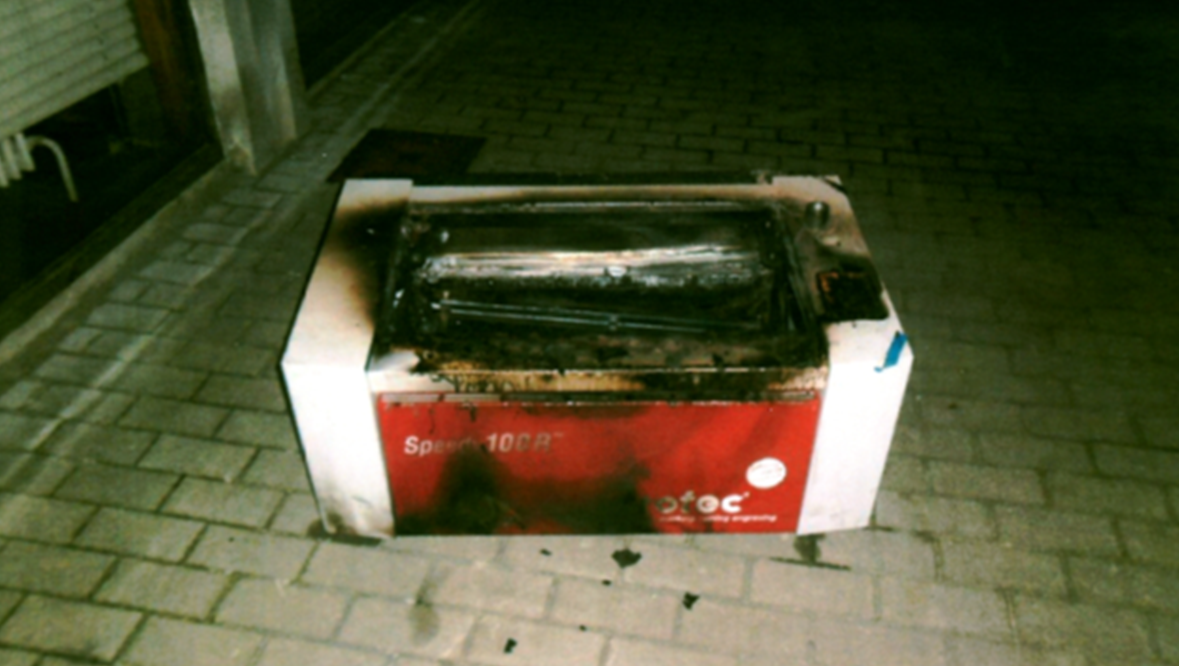
\includegraphics[width=.75\linewidth]{./img/laser-abgebrannt_fablab_leuven.jpg}
	% Mit freundlicher Erlaubnis von Marc Lambaerts, KU Leuven
	
	Bild: Ein ausgebrannter Lasercutter des FabLab Leuven. Der Benutzer meinte, weil die Datei dreimal funktioniert hat, müsse man beim vierten mal nicht mehr dabeibleiben.
	
	
	
	\vspace{5em}
	\hrule
	
	Alles bis hier musst du auswendig wissen. Den Rest kannst du bei Bedarf nachschauen.
	\vspace{0.2em}
	\hrule
	\vspace{3em}
	
	\newpage %Sieht ein bisschen schöner aus
	
	\section{Materialien}
	Wenn dein Material nicht in der Liste seht ist es nicht erlaubt! Solltest du dir aber sicher sein, dass du das trotzdem nutzen kannst, frage unbedingt einen Betreuer. Viele Kunststoffe sehen ähnlich aus, und Baumärkte haben schon oft falsche Sorten verkauft, weshalb Kunststoff ohne eindeutige Beschriftung nicht gelasert werden darf.
	
	\subsection{Erlaubt}
	\newcommand{\itemCheck}{\item[\checkmark]}
	\begin{itemize}
		\itemCheck unbrennbares zum Gravieren: Metall, Glas, Keramik, Stein
		\itemCheck dünne Lackschichten auf Metall (außer Teflonbeschichtung)
		\itemCheck erlaubte Kunststoffe: Acrylglas (PMMA), PET (Overheadfolie, Bayer Vivak), Moosgummi (EVA-Schaum), POM (Polyoxymethylen, Delrin)
		\itemCheck Papier, Pappe, Holz (auch Sperrholz, MDF, HDF und ähnliche Werkstoffe nur aus Holz und Leim)
		\itemCheck \enquote{trockene} Nahrungsmittel, soweit bekannt, wie zum Beispiel Äpfel (nur gravieren), Butterkeks ohne Schokolade, Brezen, ...
		\itemCheck PE Polyethylen / PP Polypropylen: Schaumstoffe gehen gut, Platten schlecht laserbar aber trotzdem erlaubt
		\itemCheck PS Polystyrol bis 1mm Dicke
		\itemCheck PC Polycarbonat bis 1mm Dicke
		\itemCheck spezieller laserbarer Stempelgummi aus dem FabLab
		\itemCheck Heißlaminierfolie \emph{nur} wenn sie laut Datenblatt des Herstellers aus PET+EVA besteht\\(keine Kaltlaminierfolie, diese enthält oft PVC!) 
		\itemCheck Baumwolle (auch Viskose), Leinen
		\itemCheck Bastelfilz, wenn aus Viskose oder Viskose-Wolle-Mischung (Wolle stinkt beim Lasern)
	\end{itemize}
	
	\newpage % Seitenumbruch, damit die ganze Verbotsliste zusammenhängend auf einer Seite ist
	
	\subsection{Verboten}
	\newcommand{\itemCross}{\item[$\times$]}
	\begin{itemize}
		\itemCross im Zweifelsfall: alles was nicht erlaubt ist
		\itemCross nicht eindeutig identifizierbare Kunststoffe (\enquote{irgendwas durchsichtiges})
		\itemCross spritzendes oder stark wässriges Material (Schokolade, ...)
		\itemCross ABS, Epoxidharz (GFK, CFK, Platinen), weil es übelst stinkt
		\itemCross PS Polystyrol / PC Polycarbonat dicker als 1\,mm, weil es beim Lasern spritzt
		\itemCross PA Polyamid / PU Polyurethan / Textilien mit Nylon- oder Elastan-Anteil / NBR-Gummi Nitrilkautschuk / alle Stoffe, die gleichzeitig H-, C- und N-Atome enthalten: entwickelt Blausäure (HCN)
		\itemCross halogenhaltige Kunststoffe: PVC = Vinyl = Neopren, PTFE = Teflon (z.B. als \enquote{glitschige} Beschichtung von Taschenmessern), PFA, ...
	\end{itemize}
	
	\section{Grundlagen}
	Der Lasercutter hat zwei Laser: Einen roten Laserpointer, der weitestgehend harmlos ist. Dieser ist wie ein Laserpointer ungefährlich, solange man man den direkten Strahl (z.B. mit einem Spiegel) höchstens für sehr kurze Zeit betrachtet. Das Betrachten des roten Punkts auf einem Objekt ist harmlos.
	
	Der eigentliche Laser (Infrarot mit hoher Leistung) wird sofort abgeschaltet, wenn Schutzscheibe oder Frontklappe geöffnet sind. Von ihm geht keine Gefahr aus, solange die Schutzschalter nicht manipuliert werden. Daher: keine Magneten an der Vorder- und Oberseite des Lasercutters anbringen. Desweiteren sind Magnete innerhalb des Lasercutters auch verboten!
	
	\section{Datei erstellen}
	Lege mit einem Vektorzeichenprogramm (Inkscape, Corel Draw, Adobe Illustrator) die Datei an. Je nach Programm unterscheidet sich das Vorgehen etwas:
	
	\subsection{Inkscape + VisiCut (empfohlen)}
	Wenn du Inkscape verwendest, wähle möglichst folgende Aufteilung, damit du es direkt in VisiCut weiterverarbeiten kannst.
	
	\textbf{Schneiden}: Pfade mit Linienfarbe rot, Liniendicke ist egal, keine Füllung.
	
	\textbf{Gravur}: Schwarz, Graustufen, oder beliebige Pixelgrafiken (Fotos).
	
	\textbf{Linie markieren}: Linienfarbe grün, keine Füllung.
	
	\textbf{Kommentare}: Linienfarbe oder Füllung blau. So kannst du z.B. Erklärungstexte mit in deine Datei einbauen, die nicht gelasert werden sollen.
	
	Bringe die Datei als SVG mit. Wenn du Schriftarten verwendest, die wir im FabLab nicht installiert haben, wandle den Text in Pfade um.
	
	%Du kannst VisiCut auch auf deinem eigenen Rechner installieren.
	
	\subsection{Corel Draw, Adobe Illustrator, ... + VisiCut}
	\label{corel-illustrator-svg-visicut}
	Verfahre wie bei Inkscape beschrieben, und zusätzlich:
	
	\begin{itemize}
		\item Setze den Farbraum auf RGB: zu schneidende Linien müssen echtes RGB-rot (255,0,0) sein.
		\item Wandle Text in Pfade um
		\item Corel: Beim SVG-Export die Einstellung \enquote{Formoptionen = Darstellungsattribute} setzen.
	\end{itemize}
	
	Dieses Vorgehen könnte in Zukunft einfacher werden, wenn ein Visicut-Plugin für Corel oder Illustrator fertigentwickelt wird. Wenn du daran mit entwickeln möchtest, um das Vorgehen genauso einfach zu machen wie bei Inkscape, melde dich bei uns.
	
	\subsection{Corel Draw, Adobe Illustrator, sonstiges + Windows-Druckertreiber} \label{sec:einstellungen-windowstreiber}
	Als Seitengröße müssen die Maße des Schneidtisches gewählt werden (1000 $\times$ 600~mm / \nurZing 609\,$\times$\,304~mm), da sonst Probleme auftreten können.
	
	\textbf{Vektor (Schneiden)}: Zu schneidende Linien auf eine Linienbreite von höchstens 0,001 inch stellen (Inkscape: 0,1 px, Corel Draw: Haarline, Adobe Illustrator: 0,1 px, Vectorworks: 0,03 mm). Bei fertigen Zeichnungen aus dem Internet ist Vorsicht geboten, manchmal sind hinter gefüllten Flächen solche dünnen Linien versteckt, die dann durchgeschnitten werden.
	
	\textbf{Raster (Gravur)}: Alles, das keine dünne Vektorlinie ist (sicher ab 0,25mm / 0,008 inch), wird graviert, sowohl dicke Linien und Flächen als auch Pixelgrafiken (Fotos). Die Gravur erfolgt im Graustufenmodus, sodass hellere Flächen nur leicht graviert werden, schwarze Flächen jedoch vollständig.
	
	Beim Speichern einen aussagekräftigen Namen wählen, da dieser später auf dem Display erscheint.
	
	Corel: Auf dem Rechner ws11 sind unter Nutzer fufablab08 passende Standartwerte konfiguriert.
	
	\section{Job senden}
	
	\subsection{VisiCut (empfohlen)}
	\label{VisiCut}
	
	Aus Inkscape kann man direkt über ein Plugin die markierten Zeichnungen in VisiCut exportieren. Dazu klickt man in Inkscape auf \button{Erweiterungen} / \button{Lasercut Path} %TODO in Illustrator auf ....
	. Bei Illustrator/Corel muss man ein SVG exportieren wie in \ref{corel-illustrator-svg-visicut} beschrieben und dieses direkt mit Visicut öffnen.
	
	Anschließend kann man rechts folgende Einstellungen treffen:
	
	\textbf{Material}: In der oberen Dropdown Box kann das gewünschte Material ausgewählt werden.
	
	\textbf{Stärke (mm)}: In der Dropdown Box kann die Dicke des Materials ausgewählt werden.
	
	Für jede Stärke von jedem Material speichert Visicut Lasereinstellungen. Größtenteils sind diese bereits auf sinnvolle Werte eingestellt. Prüfe diese aber unbedingt vorher auf Glaubwürdigkeit. 
	
	\textbf{Fokus}: Damit VisiCut den Fokus anpassen kann, muss es wissen wo anfangs der Fokus steht. Das Setzen des Fokus am Lasercutter wird später noch beschrieben (\cref{fokus}).
	
	\nurLTT Ändern des Fokus wird in Visicut noch nicht unterstützt. Der Fokus wird immer auf die Material-Oberseite gesetzt, dazu einfach den Autofokus ausführen.
	
	\nurZing  Normalerweise wird am Lasercutter der Fokus auf die Oberseite des Materials gesetzt, und dazu passend in VisiCut der Haken rechts bei \enquote{Fokus ist anfangs auf der Grundplatte...} \textbf{nicht} gesetzt.
	
	\textbf{Mapping (Zuordnung)}: Im Bereich Mapping kann man auswählen, wie entschieden werden soll, was geschnitten, graviert und markiert wird. Die Unterscheidung kann nach verschiedenen Kriterien erfolgen; standardmäßig wird nach Farbe entschieden: \enquote{schneide rot, graviere Rest, ignoriere blau, markiere grün}.
	
	%TODO Position
	
	\textbf{Laser Einstellungen}: Im Bereich Laser Einstellungen können die Lasereinstellungen überprüft und verstellt werden. Überprüfe vor Allem wenn es sich um ausgefallenere Materialien handelt, ob hier sinnvolle Einstellungen stehen. Oft ist es so, dass die Standardeinstellungen (Power: 0, Speed: 100, Fokus 0) gesetzt sind da diese noch nicht angepasst wurden). \textbf{Speichere deine Veränderungen nur, wenn sie auch für andere Benutzer sinnvoll sind.} Experimente bitte nicht abspeichern, sondern einfach nur den Auftrag abschicken ohne auf Speichern zu klicken.
	
	\button{Berechnen}: Dadurch wird die benötigte Zeit im Vorraus berechnet. Dies ist allerdings nur ein Richtwert und kann von der tatsächlichen Dauer abweichen. \nurLTT Wird momentan nicht unterstützt.
	
	\button{Ausführen}: Dies schickt den Auftrag an den Lasercutter. Wenn eine Erfolgsmeldung erscheint, kann der Auftrag im Laser gestartet werden.
	
	Da VisiCut in Java programmiert ist, läuft es auf jedem Betriebsystem und man kann es auch bei sich auf den Laptop installieren. Es ist verfügbar unter \url{https://download.visicut.org/}.
	
	Die aktuell verwendet Konfiguration für VisiCut kannst du beim ersten Start oder unter \verb|Optionen| / \verb|empfohlene Einstellungen herunterladen...| herunterladen. (Sie ist unter \url{https://github.com/fau-fablab/visicut-settings} in das git Repo eingecheckt. Änderungen müssen dorthin gepusht werden. Im FabLab werden auf dem Rechner beim linken Fenster des Hauptraums mit dem dortigen fu-Nutzer (\texttt{fufablab05}) die Einstellungen in einem Git-Repo abgelegt. Von dort aus können diese auf GitHub gepusht und per Pull Request mit dem Repo des FabLab abgeglichen werden. Dazu muss ein Pull Request von \url{https://github.com/FAUFabLabWS/visicut-settings} nach \url{https://github.com/fau-fablab/visicut-settings} gestellt werden. Speichere funktionierende Änderungen bitte mit dem Nutzer \texttt{fufablab05} auf dem beschriebenen Rechner ab, damit sie bei nächster Gelegenheit auf GitHub gepusht werden können. Wenn du weißt, was du tust, kannst du das Repo auch pushen. Ein passender SSH-Key für den GitHub-Nutzer FAUFabLabWS ist im \texttt{fufablab05} hinterlegt.)
	
	VisiCut ist Open Source und wird gemeinschaftlich weiterentwickelt. Wenn du Fehler findest und diese nachvollziehbar beschreiben kannst, freuen wir uns über einen Bericht an \href{mailto:kontakt@fablab.fau.de}{kontakt@fablab.fau.de} oder noch besser direkt auf github unter \url{https://github.com/t-oster/visicut/issues}.
	
	\subsubsection{Kamera} \label{kamera}

	Mit VisiCut kann man seine Vektorzeichnung auf einem Bild des eingelegten Materials platzieren. Dazu wird von einer Kamera, die an der Klappe des Lasercutters angebracht ist, ein Bild geschossen, das anhand der 4 Passermarken an den 4 Ecken der Arbeitsfläche des Lasers ausgerichtet und beschnitten wird. So können die Teile, die gelasert werden sollen, je nach Kalibrierung bis auf etwa 2mm genau am Bild ausgerichtet werden, was vor Allem bei Reststücken nützlich ist. Das Bild wird automatisch aktualisiert, es funktioniert nur wenn der Laserdeckel aufgeklappt ist.
	
	\nurLTT Es ist zu beachten, dass die Kamera noch ziemlich ungenau ist, 5-10mm Unsicherheit sind möglich! Für eine sehr genaue Ausrichtung richte dich besser nach den Linealen am Rand des Wabengitters und in VisiCut.
	
	\nurZing Vor dem Lasern ist noch zu beachten, dass der Laserkopf in den Nullpunkt des Lasercutters (links oben) zurückgefahren ist. Dazu drückt man am Laser die Taste \laserZingXyAus und danach \laserZingReset. Nach dem Start ist der Laserkopf automatisch im Maschinennullpunkt.
	
	
	\subsubsection{Fehlerbehebung}
	Sollte dies nicht funktionieren, könnten folgende Punkte hilfreich sein:
	
	%TODO Tabelle schön machen
	
	\begin{tabularx}{\textwidth}{|X|X|X|}
		\hline
		Problem		 										& mögliche Ursache															& mögliche Lösung \\ \hline \hline
		\multirow{3}{0.333\textwidth}{Das Bild wird nicht aktualisiert}	& Es wurden trotz mehrmaligen Versuchens nicht alle Passermarken erkannt	& Deckel ganz öffnen. Vergewissere dich, dass keine Marke überdeckt ist, sondern alle von der Kammera gut erkannt werden können. Eventuell ist die Kamera verdreht. \\ \cline{2-3}
		& Die Lichtverhältnisse sind zu schlecht, als dass der Kontrast zw. den weißen und schwarzen Stellen groß genug für die Mustererkennung wäre	& Schalte die Deckenbeleuchtung an oder aus\\ \cline{2-3}
		& VisiCam läuft nicht														& Frage einen Betreuer, dass er den Dienst auf der ws01 startet \\ \hline
		\multirow{2}{0.333\textwidth}{Der Laser schneidet nicht da, \\ wo er sollte}	& \nurZing War der Laser in seinem Nullpunkt und nicht links oben auf der Arbeitsfläche?	& \nurZing drücke am Laser \laserZingXyAus und \laserZingReset \\ \cline{2-3}
		& VisiCam ist verkalibriert &	Wenn du nicht an Rechner ws01 sitzt, lade aktuellere Einstellungen herunter (Optionen - empfohlene Einstellungen - Erlangen). Wenn das nichts bringt, muss auf ws01 das Kalibrierungsprogramm in VisiCut durchgeführt und dann die Einstellungen veröffentlicht werden (Betreuer/Admins fragen).  \\ \hline
		
	\end{tabularx}
	
	
	\subsection{Windows-Druckertreiber}
	
	\subsubsection{LTT iLaser}\label{sec:ltt-windows}
	Neben Visicut gibt es auch die kompliziertere Möglichkeit, den Lasercutter über einen Windows-Druckertreiber anzusprechen. Wenn möglich, verwende lieber Visicut.
	
	
	Achtung: Der Treiber darf nur von Rechner ws11 und nur mit fufablab08 Nutzer verwendet werden!
	
	Achtung: Nie zwei Leute/Fenster gleichzeitig bearbeiten, da sonst die Einstellungen überschrieben werden! \\
	Geladene Einstellungen überprüfen - bedenke dass ein falsch gesetzter Fokus Ärger bereiten kann. \\
	Scheiden = 0,03 mm rot (RGB) (0,1 funktioniert nur manchmal!)
	
	\todo{...}
	
	\subsubsection{Epilog Zing}
	
	Neben Visicut gibt es auch die Möglichkeit, den Lasercutter über einen Windows-Druckertreiber (Epilog Engraver Win32 Zing) anzusprechen.
	
	Drucken kann man nur aus Adobe Reader (Datei vorher nach PDF exportieren, geht gut für Inkscape) und Corel Draw (Import anderer Formate funktioniert nicht gescheit).  Das direkte Drucken aus anderen Programmen heraus, z.B. Inkscape, ist nicht möglich!
	
	Die Datei mit Adobe Reader bzw.\  Corel Draw öffnen, die Freigabe ist unter Computer$\rightarrow$Z:\textbackslash \ zu finden. Bei Datei$\rightarrow$Drucken \textit{Epilog Engraver} auswählen und in den Druckereinstellungen alles auf das aktuelle Material einstellen - wenn die Materialeinstellung bei Power auf 0 steht, frage einfach einen Betreuer:
	
	\textbf{Erprobte Einstellungen} können unter Erweitert geladen werden. Gute Startwerte findest du auch im Wiki (\url{http://fablab.fau.de/wiki/technik/lasercutter}). Bitte schreibe bei neuen Materialien auf, was du gewählt hast (auch die dpi-Einstellung), und ob die Werte gut funktioniert haben. Gut funktionierende Werte bitte unter aussagekräftigem Namen abspeichern, nicht funktionierende Voreinstellungen notieren und evtl.\  löschen.
	
	\textbf{Modus}: \textbf{Raster} graviert alles, das keine Haarlinie ist. \textbf{Vektor} schneidet alle Haarlinien. \textbf{Kombiniert} macht beides nacheinander.
	
	\textbf{3D-Gravur} setzt die Helligkeitsstufen des Vorlage nicht in Punktdichten (wie in Zeitungen, entspricht der Farbe der gravierten Fläche), sondern in Leistungsdichten um. Das heißt, dass eine Schwarze Fläche tiefer als eine graue Fläche graviert wird.
	
	\textbf{Stempel} ist in Kapitel \ref{stempel} dokumentiert.
	
	\textbf{Leistung und Geschwindigkeit} kann man getrennt für Vektor und Raster einstellen. Die Wirkung der Rastergeschwindigkeit hängt außerdem auch von der gewählten Auflösung ab: 500dpi reichen für normale Schrift, 1000dpi brauchen deutlich länger und sind nur für feinste Muster nötig. Bei Vektor kann man noch die \textbf{Frequenz} (Anzahl der Laserpulse pro 2,5cm Schnittlänge) einstellen. Normalerweise sollte man 5000~Hz verwenden, bei Holz und kohlenden Materialien ggf. weniger. 10~Hz kann zum Perforieren von Papier verwendet werden. %TODO ausprobieren 1000dpi vs 500dpi bei sonst gleichen Rastersettings; Vektor Frequenz
	
	\textbf{Vektoren sortieren} beinflusst, in welcher Reihenfolge die Vektoren abgefahren werden:
	\begin{itemize}
		\item \textbf{Inside-Out} schneidet zuerst innenliegende Löcher und danach äußere Konturen.  Das ist praktisch für Dinge, die beim Ausschneiden runterfallen oder verrutschen, und deshalb die übliche Einstellung.
		\item \textbf{Optimal} schneidet zeitoptimiert von links oben nach rechts unten.
		\item \textbf{Aus}: Ohne "Vektoren sortieren" wird in der Reihenfolge geschnitten, in der das Grafikprogramm die Polygone liefert, was meistens nicht optimal ist.
	\end{itemize}
	
	
	Wenn \textbf{Mittelpunkt-Definition} ausgeschaltet ist, entspricht die linke obere Ecke der Seite genau dem Nullpunkt im Lasercutter, der dann ebenfalls links oben gewählt wird. Somit kann man einfach abmessen, wo auf dem Material der gewünschte Platz ist, und in der Zeichnung die Objekte entsprechend positionieren.
	
	Ist \textbf{Mittelpunkt-Definition} aktiviert, so liegt der Nullpunkt stattdessen am Mittelpunkt der Seite (\textbf{Seiten\-mitte}) oder an einem bestimmten Punkt der benutzten Fläche (\textbf{Mitte-Mitte}, \textbf{Oben-Mitte} oder \textbf{Links-Mitte}). Dann muss man beim Lasercutter den Nullpunkt entsprechend anders legen, was später noch beschrieben wird.
	
	Auf der folgenden Zeichnung ist dies dargestellt: Der dick umrandete Kasten ist die Seite, gestrichelt ist die benutzte Fläche eingezeichnet. Das rote \textbf{x} ist an genau der Stelle, an der der Nullpunkt landet. Dementsprechend müsst ihr den Startpunkt auf dem Material platzieren.
	
	\newcommand{\mittelpunktsZeichnung}[3]{
		%\parbox{5cm}{
		\begin{center}
			\includegraphics[width=4.5cm]{#3} \\
			\textbf{#1} \\ {#2}
		\end{center}
		%}
	}
	\begin{tabularx}{\textwidth}{XX}
		\mittelpunktsZeichnung{Normal}{(Mittelpunkt-Definiton ausgeschaltet)}{./img/mittelpunkt-aus.pdf} &
		\mittelpunktsZeichnung{Seitenmitte}{für Spezialfälle - die Seitengröße kann auch entsprechend kleiner gewählt werden}{./img/mittelpunkt-seitenmitte.pdf}
	\end{tabularx}
	\begin{tabularx}{\textwidth}{XXX}
		\mittelpunktsZeichnung{Links-Mitte}{für Beschriftungen, z.B. in x-Richtung liegende Kugelschreiber}{./img/mittelpunkt-linksmitte.pdf} &
		\mittelpunktsZeichnung{Oben-Mitte}{für Beschriftungen, z.B. in y-Richtung liegende Kugelschreiber }{./img/mittelpunkt-obenmitte.pdf} &
		\mittelpunktsZeichnung{Mitte-Mitte}{für Beschriftungen}{./img/mittelpunkt-mittemitte.pdf}
	\end{tabularx}
	
	%\end{figure}a
	
	
	Wenn alle Einstellungen passen, Lasercutter einschalten (rechts hinten am Gerät). Zum Absenden des Auftrags auf OK und dann auf Drucken klicken.
	
	\section{Job ausführen}
	
	\subsection{Material}
	Material gibt es im Lagerregal und in den Schubladen nebenan in der Elektrowerkstatt. Platten kann man einfach auf den Schneidetisch legen, entstehender Rauch wird dann nach unten und hinten abgesaugt. Nach dem Job kurz warten, damit verbleibende Dämpfe abgesaugt werden. 
	
	(An den Stellen, an denen der Laser auf das Gitter trifft, gibt es beim Schneiden Reflexionen, die z.B. bei durchsichtigem Acryl störende kleine Macken an Schnittkanten erzeugen können. Um dies zu umgehen, kann man Abstandshalter unterlegen, muss dann aber aufpassen dass diese richtig platziert sind und nicht brennen.)
	
	\subsection{Bezahlung}
	\label{sec:bezahlung}
	% Bild ist obsolet:
	% \begin{wrapfigure}{r}{8cm}
	%   \vspace{-20pt} %WORKAROUND: Nicht so viel leerer weißer Platz
	%   \includegraphics{./img/bezahlung-flaeche.pdf}
	%   \vspace{-20pt} %WORKAROUND: Nicht so viel leerer weißer Platz
	% \end{wrapfigure}
	Das Material wird nach ganzen, halben (längs/quer) und viertel Platten abgerechnet. Angefangene, bereits bezahlte Platten aus der Resteschublade kosten nichts. Zusätzlich kostet die Maschinen\-zeit noch, um die Wartung der Laser\-röhre (ca. \EUR{3000} alle 5 Jahre!), den Austausch des Absaugungsfilters sowie sonstige Reparaturen und die Abschreibung zu finan\-zieren.
	Die Preise sind im Kassenterminal oder auch online (\url{https://brain.fablab.fau.de/build/pricelist/price_list-Laser.html}) verfügbar.
	
	\subsection{Fokus} \label{fokus}
	Der Laserstrahl wird durch die Linse im Schlitten auf einen bestimmen Punkt fokussiert. Damit das Material richtig geschnitten wird, muss der Tisch auf den richtigen Abstand zur Linse gebracht werden.
	
	Vergewissere Dich, dass der Laser bereits eingeschaltet und an die Nullposition (hinten rechts) gefahren ist.
	Öffne den Glasdeckel des Lasers.
	Lege Dein Material vorsichtig auf den Wabentisch und richte es aus. Der Wabentisch ist sehr empfindlich. Stütze Dich nicht darauf ab und lege keine schweren Materialien auf den Tisch. Achte immer darauf den Autofokus zu nutzen.
	
	\subsubsection{\nurLTT}
	\textbf{Achte zu jeder Zeit darauf, dass sich der Laserkopf in seiner Ebene frei bewegen kann, ohne dabei gegen irgendwas zu stoßen!} Fahre den Tisch mit der Taste \laserKnopf{Table $\downarrow$} weit genug herunter, sodass sich der Laserkopf frei bewegen kann und nicht seitlich gegen das Material stößt. Du kannst den Laserkopf jetzt mit den Richtungstasten bewegen (rund um die Haus-Taste). Um den Laserkopf sehr schnell zu bewegen, gibt es auch die Tasten P1 (Position hinten rechts) oder P2 (Position mitte Lasertisch).
	
	Bewege den Laserkopf so, dass der Fokusstift (rechts am Laserkopf) über der höchsten Stelle des Materials steht. \textbf{Vorsicht bei unebenem Material:} Wähle unbedingt die höchste Stelle -- wenn das Material woanders mehr als ca. 3mm höher ist, wird es später zu einer Kollision kommen, weil der Laserkopf am Material hängen bleibt!
	
	Drücke nun die Taste \laserKnopf{Fokus (Lupe)}. Der Laser fragt auf dem Display nun: \laserDisplay{Are you sure? Yes / No}. Bestätige mit
	\laserLTTOkay. Der Laser beginnt nun mit dem Fokussierungsvorgang. Bleibe mit der Hand an der Notaustaste, damit du gleich anhalten kannst, wenn etwas nicht in Ordnung ist und der Laser in den Tisch rumpelt. Der Laser fährt nun mit dem Fokusstift bis zum Material und dann wieder hoch.
	
	Wenn alles richtig ist, steht der Fokusstift jetzt etwa 5 Millimeter über dem Material und kann sich in der Ebene frei bewegen, ohne gegen irgendwas zu stoßen.
	
	\textbf{Sollte der Laser ausgeschaltet werden (auch Not-Aus) und dann in einer Position stehen, bei der Laserkopf nicht in der (XY-)Ebene frei bewegt werden kann, wende dich an einen Betreuer, dass vor erneutem Einschalten der Tisch per Hand heruntergefahren wird. Auf keinen Fall den Laser vorher einschalten, denn er fährt dann automatisch in die Home-Position!}
	
	\subsubsection{\nurZing} \label{fokus-zing}
	Am Linsenschlitten ist eine Pendelfeder angebracht, mit der der richtige Abstand zur Brennebene gemessen werden kann. Dort wo das Pendel im herunter geklappten Zustand endet, ist der Laserstrahl fokusiert.
	
	Dazu muss man \laserFocus drücken, das Pendel herunter klappen und dann die gewünschte Höhe mit \laserPfeilRauf/\laserPfeilRunter einstellen. Wenn man den Fokus an einem speziellen Punkt setzen möchte, kann man auch \laserZingXyAus wählen und dann den Kopf an diese Stelle schieben. Abschließen kann man den Vorgang mit \laserZingReset.
	
	\begin{wrapfigure}{r}{4cm}
		%\vspace{-50pt} %WORKAROUND: Nicht so viel leerer weißer Platz
		\includegraphics[width=4cm]{./img/focus.pdf}
		%\vspace{-20pt} %WORKAROUND: Nicht so viel leerer weißer Platz
	\end{wrapfigure}
	
	Es gibt 3 übliche Einstellungen:
	\begin{itemize}
		\item Wenn man VisiCut verwendet, kann man den Fokus auf die Grundplatte einstellen. Das ist besonders hilfreich, wenn man nacheinander verschieden dicke Materialien bearbeiten möchte, da man dann nur beim ersten mal den Fokus einstellen muss. Alles Andere übernimmt das Programm. Dazu den Haken ``Fokus ist anfangs auf der Grundplatte statt auf dem Material'' in VisiCut nicht vergessen.
		\item Wenn man nur schneiden möchte, empfiehlt es sich, den Fokus auf etwa die Hälfte der Materialhöhe einzustellen.
		\item Beim Gravieren dagegen ist es sinnvoll, den Fokus auf die Materialoberfläche zu setzen.
	\end{itemize}
	
	
	
	\subsection{Absaugung}
	\label{sec:absaugung}
	% Die Absaugung sollte in diesem Dokument nur Absaugung, nicht "Gebläse" oder "Lüftung" genannt zu werden, um Verwechslungen mit Air Assist zu vermeiden.
	
	\nurLTT Die Absaugung mit Filter ist gegen Flammenbildung, Rauch und unangenehmen Geruch, und geht automatisch zusammen mit dem Lasercutter an. Du kannst also hier nichts falsch machen. (Sie besteht aus zwei Teilen: Die Lasercutter-Absaugung wird mit dem Drehschalter vorne am Lasercutter aktiviert und pustet die Dreckluft vom Lasercutter in das Lüftungsrohr. Eine Steuerleitung aktiviert wiederum auch die Decken-Absaugung, die aus dem Lüftungsrohr absaugt und zum Dach hinauspustet. Dass die Decken-Absaugung aktiv ist, sieht man an grünem Licht am Steuerkästchen in der Ecke des Raumes, in der das Lüftungsrohr in die Decke mündet.)
	
	\nurZing Je nach Aufstellungsort wird eine externe Absauganlage verwendet, die vorher angeschaltet werden muss.
	
	%Mit der Fernbedienung kann man die Absaugung schalten (\lueftungOn/\lueftungOff) und die Geschwindigkeit festlegen (Prozentwert eingeben und \lueftungEnter  drücken bzw. \lueftungPlus/\lueftungMinus  verwenden). Für stark rauchende Materialien wie Sperrholz sollten höhere Geschwindigkeiten verwendet werden. Um die Absaugung zu verbessern, empfiehlt es sich, größere freie Flächen des Schneidetischs abzudecken.
	
	\subsection{Air Assist}
	\label{sec:air-assist}
	Da besonders bei Acryl auch mit Absaugung öfters Flammen entstehen, sind im Arm Ausströmer für Druckluft verbaut, die entstehende brennbare Dämpfe wegpusten, bevor sich eine Flamme bildet. Der Air Assist wird normalerweise automatisch mit dem Lasercutter mit angeschaltet. 
	
	Optimale Einstellung für den Druckminderer sind etwas unter 2\,bar. Dies ist normalerweise bereits korrekt eingestellt und darf nicht durch den Nutzer verändert werden.
	
	\nurZing Der Air Assist kann über einen Schalter deaktiviert werden, dann geht als Warnung automatisch auch das Licht im Lasercutter mit aus. \textbf{Für Acryl, Sperrholz und ähnliches ist der Air Assist unbedingt notwendig! Wenn er ausgeschaltet wurde (Licht im Laser aus), muss er nach dem Lasern sofort wieder eingeschaltet werden!}
	
	\nurZing Je nach Aufstellungsort wird ein externer Kompressor verwendet, der vorher angeschaltet werden muss.
	
	\subsection{Nullpunkt} \label{nullpunkt}
	\subsubsection{\nurLTT}
	Standardmäßig wird der Maschinennullpunkt verwendet: Die linke obere Ecke des Tisches entspricht der linken oberen Ecke der Seite und passt zum Kamera-Bild in Visicut.
	
	Es kann auch ein temporärer Nullpunkt gesetzt werden. (VisiCut: noch nicht unterstützt, Windowstreiber: \todo{}).
	
	\subsubsection{\nurZing}
	Bei der Nullpunktfestlegung ist besondere Vorsicht erforderlich! Wird der Nullpunkt falsch festgelegt, kann es vorkommen, dass der Lasercutter beim Ausführen des Jobs dann gegen die Begrenzung fährt und beschädigt wird. Entsprechend der Einstellung bei der Mittelpunkt-Definition muss hier der Startpunkt auf dem Material festgelegt werden.
	
	Wenn er nicht bereits angeschaltet ist, den roten Laserpunkt mit \laserRoterLaser  anschalten.
	
	Mit \laserZingXyAus deaktiviert man den Antrieb, sodass man nun von Hand den Arm (y-Richtung) und den darin befindlichen Linsenschlitten (x-Richtung) bewegen kann. Um die unten am Schlitten befestigte Linse nicht zu berühren, den Schlitten nur mit dem Zahnriemen bewegen, der oben durch den Arm läuft.
	
	Die Position des Nullpunkts überprüfen und mit \laserZingStart  bestätigen. Das Display zeigt \laserDisplay{Set Home/Center} (Nullpunkt gesetzt).
	
	Anstatt den Nullpunkt selber zu wählen, kann man auch den Maschinennullpunkt (linke obere Ecke des Tisches) verwenden. Dazu drückt man \laserZingReset anstatt Start, der Lasercutter sucht dann den Nullpunkt und fährt anschließend den Arm aus dem Weg. Für VisiCam ist das das präferierte Vorgehen (siehe Kapitel \ref{kamera})
	
	%TODO Aufschreiben: zu Maschinennullpunkt Ausmessen, in der Datei genau so hinschieben,... etc
	
	\subsection{Job laden}
	\subsubsection{\nurLTT}
	Der Laser wechselt nicht automatisch auf den neuesten Auftrag, du musst diesen erst auswählen.
	
	Wähle dazu im Display \laserLTTExit~ \laserDisplay{$\textcolor{gray}{\blacksquare}$ 1. WORK DISPLAY} \laserLTTOkay. Sende deine Datei und wähle diese im Display mit den Tasten \laserLTTPreviousJob und \laserLTTNextJob aus. Die zuletzt gesendete Datei hat die höchste Nummer, bereits ausgeführte Aufträge sind mit \texttt{*} markiert.
	
	\subsubsection{\nurZing}
	Mit \laserJob zeigt man Dateiname und laufende Nummer des aktuellen Druckauftrags an. Bei angeschalteter Mittelpunkt-Definiton wird zusätzlich \texttt{*} hinter dem Dateinamen angezeigt. Wenn der neue Auftrag nicht im Display steht, \laserZingReset drücken. Eventuell musst du auch erst etwas warten.
	
	Die Data-Leuchte muss ausgegangen sein, bevor man startet. Ansonsten sind die Daten noch nicht vollständig übertragen.
	
	\subsection{Ausführen}
	Wenn du dir unsicher bist, den Deckel öffnen, um einen Testlauf ohne Laser durchzuführen. (Lasercutter fährt den Pfad ab, doch er lasert nicht) Man sollte sich dabei nicht davon verunsichern lassen, dass der Laser beim Gravieren bis zu 3,5cm (\nurZing: etwa 5\,cm) links und rechts über das Gebiet hinausfährt, um abzubremsen und wieder in die andere Richtung zu beschleunigen.
	
	\subsubsection{\nurLTT}
	Start des Auftrags mit \laserLTTPause.
	
	Wenn der Lasercutter Unfug macht, im Zweifelsfall den Not-Aus-Schalter betätigen.
	
	\textbf{\underline{Bei brennbaren Materialien immer beim Lasercutter bleiben!}} Wenn der Auftrag abgeschlossen ist, piept der Lasercutter und zeigt die Laufzeit an.
	
	Falls der Laser nicht mehr weiter lasern soll, öffne den Glasdeckel des Lasers etwas. Der Laser fährt dann weiter. Bei Gefahr drücke die Notaustaste und rufe einen Betreuer.
	
	Wenn keine Eile besteht, kannst du den Auftrag auch pausieren, das braucht aber etwas und funktioniert manchmal nicht: Drücke 1x fest auf die Taste \laserLTTPause und warte ab. Manchmal fährt der Laser wieder in die Homeposition. Manchmal auch nicht. Im zweiten Fall ist es besser, Du wartest weiter ab.
	Ist der Laser an seine Homeposition gefahren, musst Du nun noch die Taste \laserLTTStop drücken, damit der augenblickliche Auftrag zurückgesetzt wird. Jetzt ist der Laserauftrag abgebrochen.	
	
	\subsubsection{\nurZing}
	Zum Starten auf \laserZingStart drücken (Finger weg aus dem Verfahrbereich des Laserarms!).
	
	Bei Druck auf \laserZingStop hält er am Ende der aktuellen Linie an. Dann muss man zuerst warten, bis der Lasercutter stehen bleibt. Erst sobald er wieder steht darf man entweder mit \laserZingStart fortsetzen oder mit \laserZingReset  den Auftrag abbrechen und zum Startpunkt zurückkehren. \textbf{Achtung: Wenn man nicht wartet bis der Laser steht und vorher etwas anderes drückt, kann es zu unkontrollierten Bewegungen kommen!}
	
	Wenn der Anfang des Testlaufs gut aussieht, \laserZingStop, \laserZingReset, Klappe schließen und mit \laserZingStart  den Auftrag starten. \textbf{\underline{Bei brennbaren Materialien immer beim Lasercutter bleiben!}} Wenn der Auftrag abgeschlossen ist, piept der Lasercutter und zeigt die Laufzeit an.
	
	\section{Fertigstellen}
	\subsection{Bezahlung}
	Am Display wird die Laufzeit angezeigt. Geld für Laufzeit und Material wie in~\ref{sec:bezahlung} beschrieben am Kassenterminal zahlen.
	
	\subsection{Aufräumen}
	\begin{itemize}
		\item Werkstück und Reste aus dem Bauraum entfernen.
		\item Werkzeug und Materialreste aufräumen, nicht beim Laser herumliegen lassen.
		\item Wenn mehr als eine Handvoll Reste im Schneidetisch liegen, diesen ausleeren: 
		
		\nurLTT Deckel und vordere Tür des Lasercutters öffnen. Schublade aus dem Schneidetisch herausziehen und entleeren. Schublade wieder einschieben.
		
		\nurZing Schneidetisch einfach herausnehmen (dazu müssen keine Schrauben gelöst werden). Vorderklappe des Schneidetischs entfernen (grüne Rändelschrauben lösen) und den Schneidetisch entleeren. Dann den Schneidetisch wieder zusammenbauen und so in den Lasercutter einsetzen, dass er fest sitzt.
		\item Vor dem Ausschalten des Lasers gegebenfalls die Lüftung etwas nachlaufen lassen.
	\end{itemize}
	
	\pagebreak
	
	\section{Arbeitsablauf}
	Dieses Diagramm fasst den Arbeitsablauf am Laser zusammen. Wer Probleme mit dem Lesen von Flowcharts hat, kann hier nachlesen: \url{https://xkcd.com/518/}
	
	\label{ArbeitsablaufFlowchart}
	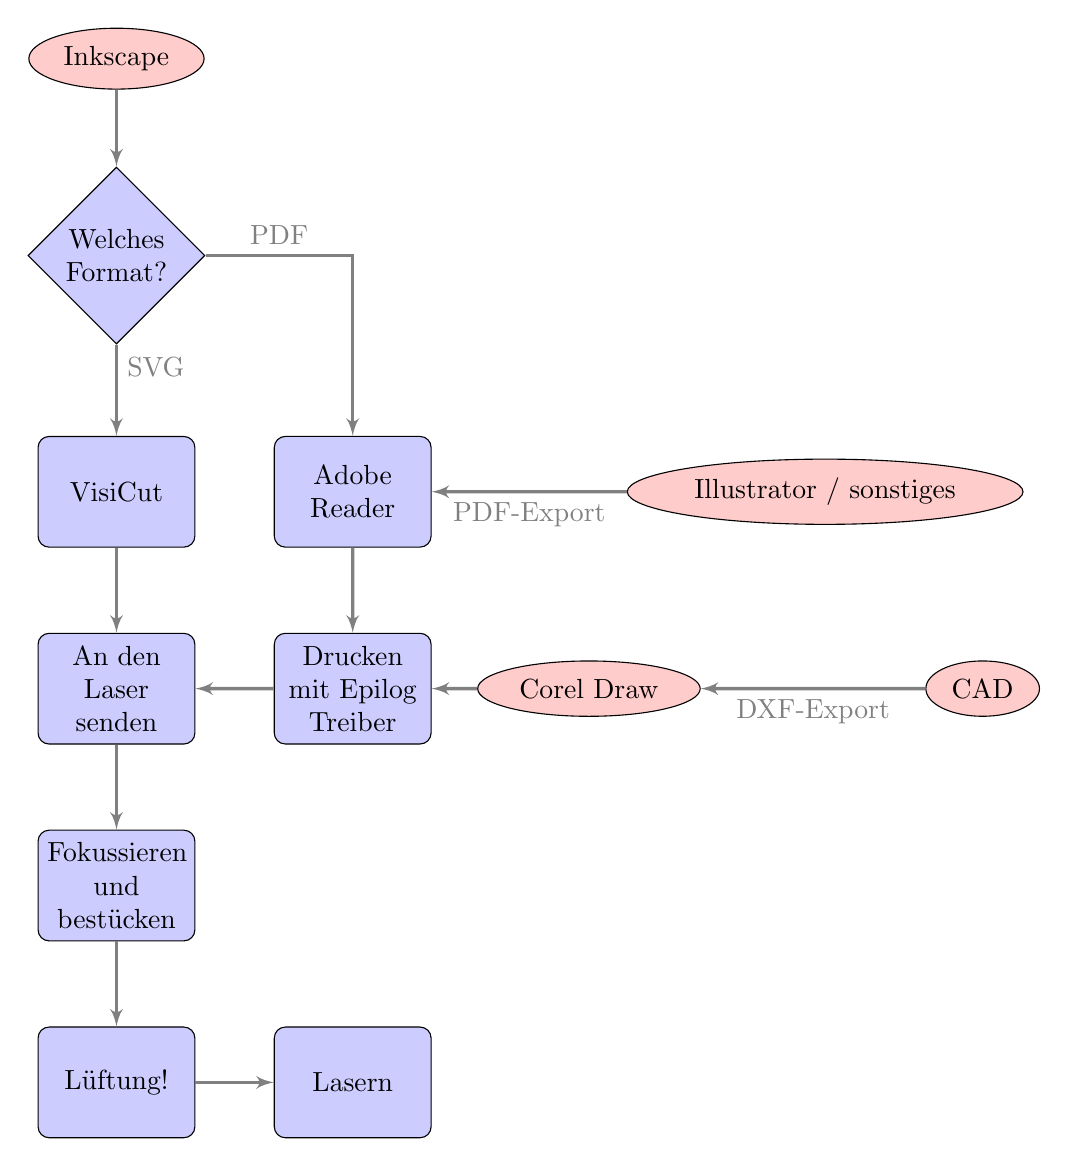
\begin{tikzpicture}[scale=0.8, node distance = 2.5cm, auto]
	%nodes, loosely sorted bottom to top
	\node [block] (luft) {Lüftung!};
	\node [block, right of=luft, node distance=3cm] (laser) {Lasern};
	\node [block, above of=luft] (fokus) {Fokussieren und bestücken};
	\node [block, above of=fokus] (uebertragen) {An den Laser senden};
	\node [block, above of=uebertragen] (visicut) {VisiCut};
	\node [decision, above of=visicut] (i_format) {Welches Format?};
	\node [cloud, above of=i_format, node distance=2.5cm] (inkscape) {Inkscape};
	\node [block, right of=uebertragen, node distance=3cm] (drucker) {\enquote{Drucken} mit Epilog Treiber};
	\node [block, right of=visicut, node distance = 3cm] (pdf) {Adobe Reader};
	\node [cloud, right of=drucker, node distance=3cm] (corel) {Corel Draw};
	\node [cloud, right of=corel, node distance=5cm] (cad) {CAD};
	\node [cloud, right of=pdf, node distance=6cm] (anderes) {Illustrator / sonstiges};
	%paths
	%decision i_format
	\path [line] (i_format) -- node [near start] {SVG} (visicut);
	\path [line] (i_format) -| node [near start] {PDF} (pdf);
	%inkscape
	\path [line] (inkscape) -- (i_format);
	%luft
	\path [line] (luft) -- (laser);
	%fokus
	\path [line] (fokus) -- (luft);
	%anderes
	\path [line] (anderes) -- node {PDF-Export} (pdf);
	%visicut
	\path [line] (visicut) -- (uebertragen);
	%pdf
	\path [line] (pdf) -- (drucker);
	%cad
	\path [line] (cad) -- (corel) node[midway,below] {DXF-Export};
	%corel
	\path [line] (corel) -- (drucker);
	%drucker
	\path [line] (drucker) -- (uebertragen);
	%uebertragen
	\path [line] (uebertragen) -- (fokus);
	
	\end{tikzpicture}
	
	%alte Version, gefällt mir grad nicht mehr
	%\begin{tikzpicture}[scale=2, node distance = 2cm, auto]
	%    % Place nodes
	%	\node [block] (idee) {Idee};
	%    \node [decision, below of=idee] (ready?) {Zeichung schon fertig?};
	%    \node [decision, left of=ready?] (format) {Format?};
	%    \node [decision, right of=ready?] (diy) {Pogramm?};
	%    \node [block, below of=diy] (inkscape) {Zeichnung in Inkscape erstellen};
	%    \node [block, right of=diy] (corel) {Zeichnung in Corel erstellen};
	%    \node [block, below of=corel] () {}
	%    % Draw edges
	%    \path [line] (idee) -- (ready?);
	%	\path [line] (ready?) -- node [near start] {Ja} (format);
	%	\path [line] (ready?) -- node [near start] {Nein} (diy);
	%\end{tikzpicture}
	
	\section{Stempel herstellen}
	\label{stempel}
	Mit dem Lasercutter lassen sich auch gut Stempel herstellen.
	Dafür gibt es im FabLab speziellen Stempelgummi.
	Dieser lässt sich mit dem Laser tief gravieren und ausschneiden.
	
	Eine genaue Anleitung dazu gibt es unter \url{https://fablab.fau.de/project/stempel}.
	
	\section{Lessons Learned}
	
	\subsection{Boxen automatisch generieren lassen}
	
	Die Vektordaten für eine praktische Box muss man nicht selbst erzeugen. Am einfachsten geht es, wenn man einen web-basierten Gerneratoren verwendet. \\
	
	Bisher wurden gute Erfahrungen mit folgenden Seiten gemacht:
	\begin{itemize}
		\item \url{http://www.makercase.com/} \\
		Wird als Vektorgrafik ausgegeben. Pfade sind so angeordnet, dass der Laser nahe beieinanderliegende Pfade nacheinander bearbeitet (gut, da ansonsten viel Zeit durch das Verfahren des Lasers verbraucht wird)
		\item \url{http://boxdesigner.connectionlab.org/} \\
		Wird als PDF ausgegeben. Allerdings ist (wenn nicht Visicut verwendet wird) die Abfolge der Pfade eher zufällig. Somit entstehen zusätzliche Zeiten durch das Verfahren des Lasers.
	\end{itemize}
	
	
	\subsection{Schnittmuster platzsparend anordnen}
	Je nach Design kann Platz gespart werden, wenn auszuschneidende Objekte
	\enquote{ineinander} geschoben werden.
	Diese mühselige Aufgabe kann von Programmen übernommen werden.
	Beispiele sind \url{https://svgnest.com/} (im Browser) oder \url{https://deepnest.io/} (zum Installieren).
	
	
	\newpage
	\section{Hinweise für Betreuer: Wartung - Epilog Zing}
	
	\textbf{Achtung! Mache folgendes nur, wenn du wirklich Ahnung hast -- Fehler können teuer werden!}
	
	\subsection{wöchentliche Reinigung: Linse, Spiegel, Wagen}
	\begin{itemize}
		\label{linsenreinigung}
		\item Auf den Schneidetisch etwas weiches legen, z.B. ein Stück altes Sweatshirt oder eine ausgebreitete Zeitung.
		\item ggf. Schneidetisch runterfahren
		\item Linse herausschrauben, entnehmen und mit der Gewinde-Seite nach unten auf den Tisch legen.
		\item 3-5 Tropfen Linsenreiniger auf Wattestäbchen aufbringen. Nur den originalen Reiniger verwenden, dieser ist 25 Prozent Isopropanol in demineralisiertem Wasser gelöst.
		\item vom Mittelpunkt nach außen wischen, dabei das Stäbchen immer ganz leicht weiterdrehen, niemals zurückdrehen! Dreck darf nicht in die Beschichtung gekratzt werden!
		\item Dies wiederholen, bis die Linse sauber aussieht. Dabei jedes mal eine frische Seite des Wattestäbchens und neuen Linsenreiniger verwenden!
		\item Nun ein letztes mal im Zickzack die ganze Fläche abwischen.
		\item Linse vollständig trocknen lassen und wieder einbauen.
		\item Mit dem Spiegel ebenso verfahren, normalerweise ist er allerdings sauber und muss nicht geputzt werden.
	\end{itemize}
	
	% TODO
	\subsection{Wartung der Mechanik}
	%TODO  fertig machen
	Der Schneidtisch läuft auf 4 Gewindestangen. Diese müssen von Zeit zu Zeit gereinigt werden. Dazu saugt man den Innenraum und die Stangen ab und wischt mit einem alten Lappen nach. Wichtig ist, dass an den Lagern sich keine Staubklumpen sammeln. Auf die staubfreien Stangen gibt man wenige Tropfen Öl.
	%TODO Skizze der Filteranlage
	\subsubsection{Filtermatte wechseln}
	Für den Holzkasten-Filter wird eine Filtermatte F5 auf 50x66cm zurecht geschnitten.
	Wechsel: seitliche Verschlüsse öffnen, Deckel abnehmen, Filtermatte entfernen, neue Matte mit flauschiger Seite nach oben einlegen, Kasten schließen.
	
	Dieser Filter ersetzt die folgenden Unterkapitel. (Diese werden nur noch für den Messebetrieb benötigt.)
	\subsubsection{Grobfilter wechseln}
	Der Grobstaubfilter ist die Tasche auf der linken Seite. Im neuen Zustand ist er weiß. Gewechselt werden muss der Filter, sobald die Anlage wegen zu geringem Durchsatz abschaltet. Dann ist der Filter meist braun.
	
	Der Filter ist mit einem eingesteckten Gummistutzen an der Rückwand befestigt. Dieser kann einfach durch leichtes Hin und Her drehen abgezogen werden. Wichtig ist beim Wechsel nicht auf den Filter zu drücken, um ein unnötiges Stauben zu vermeiden. Sobald der Filter ausgebaut ist, schraubt man die Rohrschelle auf und trennt den Stoffteil zur Entsorgung ab. Auf das schwarze Kunststoffstück wird eine neue Tasche aufgezogen und mit der Rohrschelle befestigt.
	
	Zum Schluss wird der Filter wieder eingesteckt. Ein Grobfilterwechsel sollte zusammen mit dem Stand der Lüftungslaufzeit im Laserlogbuch vermerkt werden. (siehe Wiki-Seite des Lasers)
	\subsubsection{HEPA-Filter wechseln}
	\label{subsubsec:HEPA-Filter}
	Der Feinstaubfilter besteht aus zwei Teilen. Der obere mit Klammern befestigte Teil ist der HEPA-Filter. Der Verband aus beiden Filtern kann durch Herunterklappen des weißen Hebels und Herausziehen des schwarzen Kastens aus der Anlage entfernt werden.
	Der HEPA-Filter muss nur sehr selten gewechselt werden. Dies erkennt man daran, dass die Lamellen sehr \enquote{pelzig} aussehen. \emph{Achtung! Die Lamellen sind sehr empfindlich und dürfen nicht berührt werden.}
	Ein Wechsel des HEPA-Filters muss im Laserlogbuch zusammen mit dem Stand der Anlagenlaufzeit notiert werden.
	\subsubsection{Aktiv-Kohle-Filter wechseln}
	Der Aktiv-Kohle-Filter ist der schwarze Kasten unter dem HEPA-Filter. Zum Ausbau siehe den Abschnitt \ref{subsubsec:HEPA-Filter}.
	
	Zunächst sollte man nach dem Ausbau die untere Gummidichtung überprüfen. Diese schließt den Filter luftdicht ab und verschleißt von Zeit zu Zeit. Defekte Stellen sollten heraus geschnitten werden und durch neues P-Klebeband von Tesa Moll ersetzt werden. Dieses Band lässt sich über unser Teilesystem finden. Dabei sollten zwei Bänder so nebeneinander geklebt werden, dass sich ein Hohlraum zwischen zwei Wülsten bilden kann.
	
	Bei schlechter Filterleistung (Geruchsbildung) ist es oft ausreichend, die Aktivkohle neu aufzuschütteln. Danach kann es vorkommen, dass die Lüftung etwas Staub spuckt, also erstmal draußen betreiben.
	
	Wenn dies nichts bringt, muss die Aktivkohle gewechselt werden. Dazu entfernt man das schwarze Klebeband am oberen Rand des Filters. Dieses sollte man aufheben, da es wieder verwendet werden kann. Für die weiteren Schritte sollte nach Außen gegangen werden. Zunächst entfernt man den Deckel, welcher mit vier Ausstülpungen des Grundteiles befestigt ist. Jetzt werden die Aktiv-Kohle und die zwei Filtermatten entsorgt. Achtung! Dies staubt massiv. Den Staub nicht einatmen!
	
	Abschließend legt man eine Filtermatte in den Boden, gibt die Aktiv-Kohle darauf und legt eine Filtermatte in den Deckel. Den Deckel wieder festdrücken und mit Klebeband luftdicht verschließen. Eventuelle Lücken werden mit weiterem Klebeband gedichtet. Nun montiert man den HEPA-Filter und schiebt die Einheit wieder in die Absauganlage.
	Ein Wechsel des Aktiv-Kohle-Filters muss im Laserlogbuch zusammen mit dem Stand der Anlagenlaufzeit notiert werden.
	\subsubsection{Neue Grobfilter nähen}
	Das Material für die Filter kann bei Großhändlern quadratmeterweise bestellt werden. Das Schnittmuster gibt es im Netzlaufwerk. Beim Nähen ist es wichtig auf eine dichte Naht (Stiche nah beieinander, eventuell Overlock) zu achten. Außerdem muss man aufpassen, dass die Öffnung groß genug für den Gummistutzen ist.
	\subsection{Lasergitter reinigen}
	Durch verbrannte Holz und Acrylreste verfärbt sich das Metallgitter des Lasertisches immer weiter. Ab einem gewissen Grad färbt dieser Schmutz ab. Wenn dies eintritt muss das Gitter gereinigt werden.
	\begin{itemize}
		\item Gitter herausnehmen (mit Rahmen) und am Waschbecken bereit legen. Backofenreiniger und Heißluftpistole hohlen.
		\item Mit der Heißluftpistole das Gitter gut aufheizen. (Richtig heiß machen, jedoch nicht so heiß, dass der Lack sich ablöst!)
		\item Backofenspray schütteln und gleichmäßig von allen Seiten auftragen.
		\item Mit der Heißluftpistole weiter aufheizen. Achtung! Geruchsentwicklung! Absaugung des Raumes laufen lassen.
		\item Gegebenenfalls Prozedur wiederholen.
		\item Mit viel Wasser und wenig Sauerei ausspülen.
		\item Zwischen den Gitterblechen kann mit einem Pfeifenreiniger oder einem Tuch gewischt werden. Achtung! Das Blech lässt sich leicht verbiegen.
		\item Zum Schluss den Boden des schwarzen Gehäuses auswischen. Dabei die Hand sehr flach machen und nicht an den Gitterkanten schneiden!
		\item Gut durchtrocknen lassen und wieder einbauen. Dabei auf Ebenheit achten.
	\end{itemize}
	\subsection{ausführliche Wartung}
	%TODO
	Zur ausführlichen Wartung gehören die folgenden Punkte:
	\begin{itemize}
		\item Ausbauen des Schlittens
		\item Abwischen der Laufflächen des Schlittens (das Profil und die Rollen mit einem weichen Lappen reinigen)
		\item Prüfen der Riemenspannung von X- und Y-Achse
		\item Reinigen der Linse und Überprüfen auf Defekte
		\item Reinigen des Innenraums mit Breff Eingebrannte oder mit Industriereiniger
		\item Reinigen und Abrichten des Gittertisches
		\item Wartung der Z-Mechanik
		\item Warten der Filtereinheit
		\item Zerlegen des Absaugkasten und Ausblasen des Saugermotors
		\item weiteres siehe Wartungsliste
	\end{itemize}
	
	\subsection{Lasermatch einstellen}
	Der Lasercutter graviert die Zeilen immer abwechseld von links nach rechts und umgekehrt. Dabei kann ein leichter Versatz zwischen links- und rechtsherum gravierten Zeilen auftreten, der vertikale Gravurkanten kammförmig erscheinen lässt. Zum Testen lasert man mit 1000dpi eine feine vertikale Linke oder feine Schrift (ein kleines i in 9pt Times). Dies wiederholt man mit verschiedenen Lasermatch-Einstellungen und wählt die, bei der die Kante optimal aussieht.
	
	Details dazu stehen im Handbuch.
	
	\section{häufige Fehler}
	\label{sec:fehler-allgemein}
	In diesem Abschnitt geht es um die Beseitigung häufiger Fehler. Wenn das Werkstück fehlgeschlagen ist, werden die Laserzeitkosten des Fehlschlags in der Regel erlassen. Material muss weiterhin bezahlt werden.
	
	Hinweise speziell für LTT bzw. Zing Lasercutter finden sich in den nachfolgenden Abschnitten. Ebenso Hinweise zur Wartung für Betreuer.
	
	\subsection{Windowstreiber}
	\subsubsection{Objekt wird nicht geschnitten, sondern graviert}
	\begin{itemize}
		\item Einstellungen im Programm richtig gemacht? Siehe \cref{sec:einstellungen-windowstreiber}.
		\item Richtiges Programm verwendet? Siehe Abschnitt \ref{ArbeitsablaufFlowchart} Arbeitsablauf
		\item Liniendicke 0.1 \textbf{Pixel} bzw. Haarlinie (Corel)
		\item Inkscape: Deckkraft 100\% (Objekt $\rightarrow$ Füllung und Kontur $\rightarrow$ Schieberegler ganz unten: Deckkraft)
		\item Keine Transparenz (Alphakanal, Deckkraft) verwenden! Auch nicht in Farbverläufen.
		\item Illustrator: Gruppen mit Zuschneidepfad machen oft Probleme; diese auflösen.
		\item Achte auf deinen Farbmodus! Farbmodus auf Datei $\rightarrow$ Farbmodus $\rightarrow$ RGB
		\item PDFs werden beim Exportieren manchmal gerastert bzw. kaputtgemacht. Keinen PDF-Export aus Corel verwenden!
	\end{itemize}
	
	\section{\nurLTT Fehlerbehebung - nur für Betreuer}
	In diesem Abschnitt geht es um die Beseitigung häufiger Fehler speziell beim LTT Laser.
	Informationen zur Wartung und ernsthaften Problemen siehe Abschnitt \ref{sec:wartung-ltt}.
	
	
	\subsection{Unerwünschte Gravur am Rand}
	Wenn rechts und links von einer Gravur auch dunkle Stellen graviert werden, ist die \enquote{Tickle Power} zu hoch eingestellt. Das ist die Leistung, die bei ausgeschaltetem Laser zum \enquote{Vorglühen} der Laserröhre verwendet wird. In Rücksprache mit dem Hersteller sollte diese dann verringert werden. (Auslieferung: Tickle Frequency 20kHz, Dezember 2018: verringert auf 18 kHz, Juni 2019: 16 kHz).
	
	Zu hohe Tickle Power führt auch dazu, dass bei ausgeschaltetem Laser trotzdem Linien auf das Material markiert werden. Bei Thermopapier (Kassenzettel) lässt sich das nicht hunderprozentig vermeiden, bei anderem Material sollte es nicht vorkommen.
	
	
	\section{\nurLTT Wartung - nur für Betreuer}
	\label{sec:wartung-ltt}
	\textbf{Achtung! Mache folgendes nur, wenn du wirklich Ahnung hast -- Fehler können teuer werden!}

	Die Achsen sind: X links-rechts, Y vor-hinter, Z für den Tisch.
	
	\subsection{Handbücher des Herstellers}
	Normale Reinigung der Optik und Mechanik siehe Benutzerhandbuch des Herstellers. Problembehandlung siehe Wartungshandbuch des Herstellers. Beides liegt auf der Dateifreigabe unter Fablab / Geräte / Laser.
	
	\subsection{wöchentlich: Führungen putzen}
	Die X-Achse hat 3 Laufrollen - 1 oben und 2 unten. Die zwei Y-Achsen haben jeweils 2 Rollen. Die Rollen laufen in Führungsrillen in einem Aluprofil.
	
	Alle Rollen mit weichem Tuch abwischen. Es darf kein Alkohol o.ä. verwendet werden, dieser macht die Rollen spröde.
	
	Alle Führungsrillen (am Laserkopf oben und unten, Y ganz links, Y ganz rechts) mit Tuch und ggf. Spiritus abwischen. Es darf kein Spiritus an die Rollen gelangen!
	
	\subsection{wöchentlich: Optik putzen}
	
	Linsen reinigen:
	\begin{itemize}
		\item Am Linsenwagen die Schrauben vorne an den Ecken (grün makriert) herausschrauben.
		\item (frisches) Wattestäbchen in Linsenreiniger tunken und mit leichter rückwärts Rollbewegung die Linse putzen. Mit dreckiger Seite nicht erneut über die Linse gehen, lieber ein neues Wattestäbchen nehmen.
		\item Linse vorsichtig mit Druckluft trocknen und wieder installieren. Die gekrümmte Seite der Linse sollte oben sein, also darauf achten, den Linseneinsatz richtig herum einzusetzten (richtige Orientierung ist mit einem Aufkleber beschriftet).
	\end{itemize}

	Spiegel reinigen:
	\begin{itemize}
		\item Spiegel 5 (Spiegel im Linsenwagen)
		\begin{itemize}
			\item 	Anleitung dazu ist im Wartungshandbuch in der Freigabe unter: Dateifreigabe / 1\_fablab / 1\_Geraete / Laser / Anleitung Novograv (LTT) iLaser 4000 / Wartungshandbuch\_iLaser\_05:2018/
			\item 	Wartungshandbuch hier falsch: der Spiegel kann nicht herausgezogen werden, deshalb statdessen den Spiegel vorsichtig mit Wattestäbchen und Linsenreiniger ähnlich der Linse durch die seitliche Öffnung reinigen.
		\end{itemize}
		\item Spiegel 4 (Am Ende der Schiene, auf der der Linsenwagen fährt): Nach gleicher Methode mit Wattestäbchen und Linsenreiniger
		\item Spiegel 3 und Austrittsfenster daneben: Nach gleicher Methode mit Wattestäbchen und Linsenreiniger
	\end{itemize}

\textbf{Nach der Wartung kontrollieren, dass KEINE GEGENSTÄNDE im Laser liegen, BEVOR man ihn anschaltet, sonst Kollisionsgefahr!}
	
	Nur wenn erforderlich:
	
	Spiegel 1 und 2 kontrollieren und säubern:
	\begin{itemize}
		\item Stecker ziehen!
		\item Seitenklappe unten mit Schlüssel aus der Betreuerschublade öffnen
		\item Nach Wartungshandbuch Kapitel 4.6 (S. 16) vorgehen: Abdeckung laut Wartungshandbuch öffnen und kontrollieren ob Spiegel und Einkoppelspiegel sauber sind, NICHT verstellen.
	\end{itemize}

	
\subsection{wöchentlich: Ansauglüfter der Laser-Elektronik säubern}
	Der Lasercutter hat vier Ansaugfilter - zwei unten, zwei hinten. Wenn sich diese zusetzten verdreckt der Laser auch unten beschleunigt, da er dann dreckige Luft aus dem oberen Bereich ansaugt.
	
	 Staubsauger auf niedrigste Stufe stellen und mit etwas Abstand (!) die Filter aussaugen. Es besteht die Gefahr, dass man versehentlich den Filter einsaugt - ein Reservefilter (G2 Grobfilter, Amazon) findet sich im Gehäuse des Lasercutters unten.
	
	Normalerweise reicht das. Wenn man trotzdem von innen an die Filter und Lüfter rankommen will:
	\begin{itemize}
		\item Stecker ziehen!
		\item Seitenklappe unten mit Schlüssel aus der Betreuerschublade öffnen
		\item Lüfterfilter reinigen.
	\end{itemize}
	
\subsection{ab und zu: Riemenspannung / zittriges Schnittbild}
	Zu schwache Riemenspannung führt dazu, das das Schnittbild zittrig wird. Außerdem kann dann bei Crash einer der der Y-Riemen durchrutschen, sodass die X-Achse dann schief läuft. Zu starke Riemenspannung hingegen führt zu überhöhtem Verschleiß und letztlich einem gerissenen Riemen.
	
	Zum Prüfen der Riemenspannung immer in die Mitte der Arbeitsfläche fahren (P2). Leider gibt es vom Hersteller nur sehr vage Beschreibungen der Riemenspannung:
	
	\paragraph{Korrekte Riemenspannung der Y-Achse (links und rechts):} Bei mäßigem Druck (ca. 2\,kg) gegen die Y-Achse links/rechts (nahe an den Laufrollen mit denen sie an der Führung läuft, nicht zuweit oben in Z) soll sie sich um nicht mehr als ca 1mm bewegen.
	
	Achtung: 2kg sind weniger Druck als du denkst. (Balanciere eine Wasserflasche auf deinem Daumen, das ist etwa 1\,kg.) Nicht stärker drücken, sonst rutscht der Riemen durch und man hat großen Justieraufwand. 
	
	\paragraph{Korrekte Riemenspannung der X-Achse:} Wenn man lange genug im Wartungshandbuch sucht, findet man folgende Angabe: Der X-Riemen ist richtig gespannt, wenn er sich \enquote{in der Achsmitte ca. 1-1,5 cm von der Achse wegziehen lässt}. Nicht Übermäßig fest spannen. Y-Riemen muss 10 \% mehr Spannung haben als der X-Riemen.

\subsection{Laserleistung prüfen (bei Bedarf)}
3mm Acryl XT ohne Schutzfolie sollte bei Speed 10-11, Power 100, gerade noch durchgeschnitten werden (fällt von selber oder mit sehr leichtem Klopfen noch raus). Dies soll in allen Ecken des Lasercutters der Fall sein (meist ist es unten rechts um 1 Speed-Einheit schlechter). Ein Vergleichsmuster liegt in der Kiste mit Wartungsmaterial.

Ein Stück Acryl 3mm XT (XT hat bessere Dickentoleranzen als GS, XT ist an blauer Schutzfolie zu erkennen) einlegen und Autofokus ausführen.

Zum Testen wird VisiCut gestartet und ein spezielles LaserScript geladen, das Rechtecke mit verschiedenen Geschwindigkeiten schneidet: Datei \pfeil Beispiele \pfeil vordefiniert \pfeil LaserScript \pfeil Speedtest. Bei den Abfragen dann Maximum Speed 13, Minimum Speed 7, Step 1 eingeben und auf \enquote{Acryl, alles cut} stellen. Wenn beim Senden nochmal die Abfrage nach Speed-Werten kommt, erneut die vorherigen Werte eingeben.




\subsection{Ausrichtung der Optik prüfen (bei schlechter Leistung, obwohl sonst alles stimmt)}\label{ltt-wartung-optik}
Ziel ist, dass die Position des Laserstrahls an jedem einzelnen Spiegeln gleich bleibt, egal wie man die X- und Y-Achse bewegt. Toleranz entlang Y-Achse: Bei über 0,5mm sollte man nachjustieren, besser ist deutlich weniger. Toleranz entlang X ggf. etwas größer.

Wenn die Ausrichtung nicht stimmt, kann das auch an einer falsch ausgerichteten X-Achse liegen! Deshalb vor dem Justieren der Optik zunächst die Checkliste in \cref{sec:wartung-ltt:kollision} abarbeiten.

Es gibt ein Fadenkreuz, das an die Position der Linse eingesetzt wird. Dieses wird aus Kassenzettelpapier ausgelasert, fertige Exemplare finden sich in der Wartungskiste. Die Datei liegt in fablab-data/Maschinen/Novograv (LTT) iLaser 4000/. Die Position des Laserpunkts darauf sollte sich nicht mehr als ca. 2mm verändern, besser deutlich weniger. Mittigkeit des Laserpunkts sollte unter ca. 3mm sein, besser deutlich weniger.

Tips:
\begin{itemize}
	\item Der rote Laserstrahl passt nicht hundertprozentig zum eigentlichen infraroten. Allerdings bewegt er sich, wenn man die Optik verstellt, in die gleiche Richtung und um den gleichen Weg. Das ist sehr hilfreich um zu sehen ob man in die richtige Richtung verstellt hat. Am besten die alte Position mit einem Stift markieren.

	\item Die Stellschrauben muss man normalerweise nur äußerst wenig verdrehen. Eine viertel Umdrehung ist meist viel zu viel.
\end{itemize}

Alles weitere steht im Wartungshandbuch.

\subsection{Prüfen der Achsen nach (vermutlicher) Kollision} \label{sec:wartung-ltt:kollision}
	\begin{itemize}
		\item Netzstecker (Kaltgerätekabel) ziehen!
		\item Position Z-Achse prüfen: Kann der Laserkopf frei in der (XY-)Ebene bewegt werden? Wenn nein, musst du den Tisch vorher per Hand herunterfahren: Netzstecker ziehen (Kaltgerätekabel rechts an Laser), Wartungsklappe vorne unten mit Schlüssel öffnen (Betreuerschublade), durch Schieben des Zahnriemens den Tisch hoch/runter bewegen. Ein Hinweiszettel am Boden des Gehäuses zeigt die nötige Bewegungsrichtung für das Herunterfahren des Tisches. Wartungsklappe wieder schließen. Gerät noch nicht in Betrieb nehmen, erst die folgenden Punkte abarbeiten.
		\item Fokusstift prüfen: Muss frei herunterfallen, wenn man ihn hochhebt, und darf nicht krumm o.\,ä. sein. Etwas Spiel der Fokusstifthalterung ist normal, diese ist relativ lose am Laserwagen befestigt.
		\item Rollen X/Y prüfen: 7 Rollen (2 links an linker Y-Achse, 2 rechts an rechter Y-Achse, 2 oben an X, 1 unten an X) müssen jeweils in der V-Nut im Aluprofil laufen. Siehe Bilder im Wartungshandbuch unter \enquote{5.1 Ausrichten der Achsen - Vorbereitende Maßnahmen}. Das ist nicht einfach zu sehen, man braucht normalerweise Lampe und Spiegel/Handykamera dafür.
		
		Wenn das nicht in Ordnung, ist die Achse oder der Laserkopf ausgehängt und muss erst wieder eingehängt werden. Wenn dies nicht durch leichtes Wackeln von selber passiert, muss sie dazu teilweise demontiert werden. Siehe Wartungshandbuch unter \enquote{9. X-Achse ausgehängt}.
		\item Die Rollen dürfen nicht frei in der Luft drehen, sondern sollen auf der Nut aufliegen. Das prüft man durch vorsichtiges Drehen mit der Hand. Richtig ist es, wenn sie sich nicht frei drehen lassen ohne dass sich der Wagen bewegt, bzw. man erst etwas kräftiger drehen muss bis sie merklich durchrutschen. 	Bei allen Rollen einer Achse soll das ungefähr gleich sein.
		
		Wenn sich eine der Y-Rollen frei dreht, dann ist ziemlich sicher die Rechtwinkligkeit der X-Achse falsch. Bei der X-Achse kann sich die Rolle eigentlich nur dann frei drehen, wenn der Laserkopf nicht richtig eingehängt ist.
		

		\item Rechtwinkligkeit der X-Achse grob prüfen, zunächst bei ausgeschaltetem Lasercutter:
		
		Zum Prüfen (auf etwa $\pm$ 0,5 mm genau) werden 1-2 spezielle Justierwinkel\footnote{Dateifreigabe/1\_fablab/1\_Geraete/Laser/Justierwinkel.svg, gelasert oder idealerweise gefräst, mindestens 8mm dick} und 2-3 Stücke 0,5\,mm dicke Folie benötigt (Wartungskiste).
		
		Laserkopf vorsichtig von Hand in die X-Mitte bewegen damit er aus dem Weg ist.
		
		Y-Achse (durch Drehen am Riemenrad hinten mitte) so bewegen dass die Vorderkante der X-Achse genau über der Vorderkante des \emph{linken} schwarzen Befestigungsblocks steht (Bild). Zuerst grob nach Augenmaß, dann für die Feinjustierung den Justierwinkel anlegen:
		
		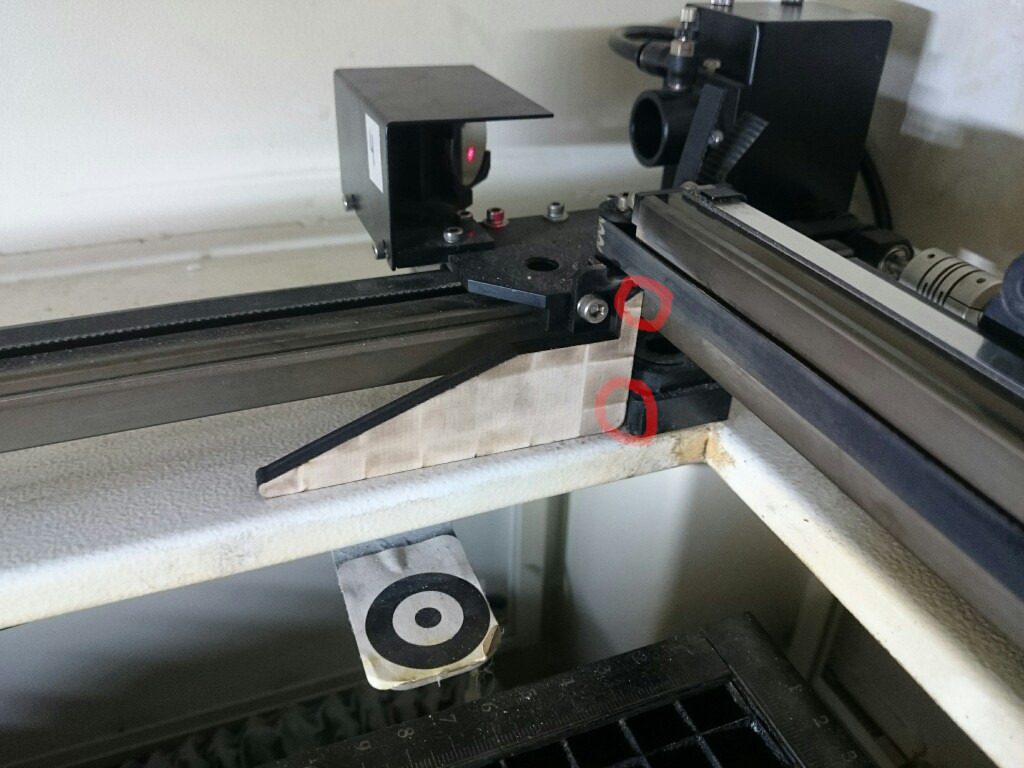
\includegraphics[width=.5\linewidth]{img/laserjustierwinkel}
		
		Der Justierwinkel liegt korrekt an, wenn man weder oben noch unten ein 0,5mm Stück Folie komplett dazwischenstecken kann.
		
		Achse so stehen lassen. Jetzt den zweiten Justierwinkel am \emph{gegenüberliegenden} (rechten) Befestigungsblock anlegen. Wenn die Achse schräg ist, ergibt sich jetzt oben oder unten ein Spalt zwischen Prüfwinkel und Achse bzw. Befestigungsblock.
		
		Wie groß der Spalt ist, kann man durch Dazwischenstecken mehrerer Folien messen. Gut sind 0,5\,mm. Schlecht sind 1,5\,mm oder mehr. Bis etwa 5\,mm kann man den Lasercutter noch gefahrlos für Justierzwecke betreiben, auch wenn er dann schon lange nicht mehr sinnvoll schneidet.
		
		\item Wenn die Abweichung über 4\,mm ist, zuerst die Rechtwinkligkeit korrigieren (siehe nächster Abschnitt). Ansonsten zunächst die nachfolgenden Punkte weitermachen bevor korrigiert wird.
		
		\item Die Lichtschranken der X- und Y-Achse prüfen. Zunächst sicherstellen, dass diese festgeschraubt und nicht lose oder abgebrochen sind. Dann von Hand die X-/Y-Achsen dort hin verschieben und sicherstellen, dass das \enquote{Fähnchen} mittig in die Lichtschranke ragt. Beide Lichtschranken sitzen rechts hinten, die zweite etwas versteckt unterhalb der ersten. Siehe Wartungshandbuch unter \enquote{10. Sensoren der Parkposition prüfen}.
		
		\item Laser wieder einschalten, prüfen dass Referenzfahrt beim Einschalten funktioniert.
		
		\item Prüfen dass die Riemenspannung grob stimmt (siehe vorher). Wenn diese nicht passt, sollte sie vor/während der Justierung der Rechtwinkligkeit korrigiert werden.
		
		\item Messung der Rechtwinkligkeit bei eingeschaltetem Laser wiederholen, so wie vorher beschrieben. Weil die Achse jetzt fest stehen bleibt, ist die Messung genauer möglich (auf ca. 0,5\,mm). Messe lieber zweimal, um Messfehler auszuschließen --- wenn man den Justierwinkel nicht flächig auf den Boden auflegt, misst man schnell 1\,mm falsch.
		
		Ist die Abweichung 1\,mm oder weniger? Dann bist du hier fertig und darfst den Laser wieder in Betrieb nehmen, und noch den Nullpunkt (\cref{sec:wartung-ltt:nullpunkt}) prüfen. Ansonsten geht es weiter mit dem nächsten Abschnitt.
	\end{itemize}
\subsection{Rechtwinkligkeit der Achsen korrigieren}
	Wenn die Prüfung (siehe vorheriger Abschnitt) zeigt, dass die Achse schräg steht, hast du etwas mehr Aufwand. 
	
	\emph{Beachte:} Wenn die Achse schräg steht, stimmt dadurch auch die Ausrichtung der Optik nicht mehr. Wird die Achse neu justiert, muss danach meist auch die Optik ein bisschen (paar Millimeter im Fadenkreuz) nachjustiert werden.
	
	Gerät ausschalten. Vorgehen wie im Wartungshandbuch unter 5.2 beschrieben, aber die Rechtwinkligkeit nicht anhand des Laserpunkts, sondern mit dem Justierwinkel (siehe vorheriger Abschnitt) bestimmen. Klemmkupplung zwischen linker und rechter Y-Achse etwas lösen sodass man sie mit etwas Widerstand verdreht werden kann. In kleinen Schritten verdrehen solange bis die Prüfung mit dem Justierwinkel erfolgreich ist. Die gesamte Achse kann man durch Drehen am Riemenrad des Motors (hinten mitte) bewegen.
	
	Klemmkupplung wieder festschrauben (ohne Gewalt!).
	
	\subsubsection*{Weitere Notizen}
	Zur Erklärung, wieso das Vorgehen laut Wartungshandbuch nicht so sinnvoll ist:
	\begin{itemize}		
		\item Der Laserstrahl ist nicht zum Ausrichten der Achse geeignet, denn der ist selber nie hunderprozentig genau justiert. Obendrein kann man die Optik erst ausrichten, wenn die Achse bereits korrekt ausgerichtet wurde. Da beißt sich die Katze also in den Schwanz.
		
		\item Die Optik (Linse) dafür, dass der Laserpunkt auf der Arbeitsfläche tendentiell andersherum schräg wandert als die Achse schräg ist. Weil Spiegel 4 mit auf der Achse sitzt, bewegt sich beim Schrägstellen der Achse der Laserpunkt etwa doppelt so weit wie die Achse selbst.
		
		\item Der rote Laserstrahl passt nie hundertprozentig zum eigentlichen Infrarotlaser, passt also noch weniger.
		
		\item Das Lineal am Wabentisch ist nicht exakt achsparallel. Das unten auf der Grundplatte ist es halbwegs, man müsste aber den Anschlag der Z-Achse temporär ausbauen um so tief fokussieren zu können. (Genau, aber für uns nicht nützlich, sind die bei Y=54.2mm auf der Grundplatte unter dem Wabentisch eingeritzten Linien. Diese wurden vom Service genau achsparallel eingeritzt, genau senkrecht zur linken Y-Achse, welche als Referenz dient.)
		
		\item Weil man die Achse nie ganz exakt wiederholgenau justiert bekommt, kann es nach Neu-Ausrichten der Achse sein, dass die Optik ein bisschen (paar Millimeter Abweichung im Fadenkreuz) nachjustiert werden muss. $\rightarrow$ \cref{ltt-wartung-optik}
	\end{itemize}

	Bei größerer Unsicherheit (sollte nicht nötig sein) kann man abschließend folgendes prüfen, nachdem Optik und Achse justiert wurden:

	\begin{itemize}
		\item Das ist leider ein relativ hoher Aufwand, weil die Z-Begrenzung verstellt werden muss.
		
		Man kann aber den Tisch nicht weit genug hochfahren, um zu testen ob der Laser zu dieser Linie passt, weil wir die Z-Achse so begrenzen, dass bei eingebautem Wabentisch man mit dem Fokusstift nicht viel tiefer als der Wabentisch fahren kann. Also muss man zunächst die Begrenzung der Z-Achse temporär entfernen, weil wir direkt auf der unteren Tischplatte \enquote{lasern} wollen. Dazu mal wieder Netzstecker ziehen, Wartungsklappe unten aufmachen, Fähnchen der Z-Achse mit 3mm Inbus aufschrauben und abnehmen, Wartungsklappe wieder zu. Strom an.
		
		Der rote Laserpointer soll beim Verfahren in X-Richtung auf der Referenzmarkierung von ganz links bis ganz rechts genau auf der Markierung bleiben und nicht nach vorne oder hinten wegwandern (Toleranz ca 0.5mm). Wenn das nicht so ist, stimmen entweder die Optik-Ausrichtung, die Justierung des roten Lasers relativ zur Optik oder die Achsausrichtung oder mehrere davon nicht.
		
		\item Nun die Z-Begrenzung wieder auf vorherigen Bereich: Tisch auf ungefähr die Höhe der vorherigen Z-Begrenzung fahren, wieder Netzstecker ziehen, Z-Begrenzung wieder einbauen: blauer Strich = Oberkante Fähnchen, sicherstellen dass das Fähnchen mittig in die Lichtschranke passt. (Die Höhe der Begrenzung ist knapp unter der Wabentisch-Höhe gewählt, dass man beim Fokussieren nicht tief im Wabentisch steckenbleiben kann, aber noch problemlos ein dünnes Blatt Papier fokussieren kann.)
		
		Wartungsklappe zu und Strom an.
	\end{itemize}

Zur Vollständigkeit hier noch das Vorgehen wie es der Hersteller vorschlägt:

\begin{itemize}
	\item Benötigt werden hierzu ein rechtwinkliges Alublech (Ein entsprechend beschriftetes lagert in der E-Werkstatt unter dem Plotter-PC-Bildschirm), zwei ca. 40mm dicke Unterlegwinkel (\todo{noch zu fertigen, siehe Fotos fablab-data/Maschinen/Novograv (LTT) iLaser 4000/Fotos Wartung 2019-04-11/ } und \url{https://cad.onshape.com/documents/bccee6264ce702916cd9ce98/w/eebe4988cdecfe89ec7acab5} ), sowie ein ebenso dicker Unterlegklotz.
	
	\item Z-Begrenzung deaktivieren wie in der vorherigen Auflistung beschrieben.
	
	\item Gerät ausschalten. Vorgehen wie im Wartungshandbuch unter 5.2 beschrieben, aber die Rechtwinkligkeit nicht anhand des Laserpunkts, sondern nach der folgenden Art bestimmen: Klemmkupplung zwischen linker und rechter Y-Achse lösen. Das Aluprofil der linken Y-Achse dient als Referenz. An dieses wird das rechtwinklige Alublech angelegt und dann gegen die X-Achse geschoben, sodass sich diese passend rechtwinklig schiebt. Damit die Verbindung der X- und Y-Achse dem Blech nicht im Weg ist, werden dabei Unterlegwinkel vor die X-Achse gelegt, und der X-Riemen wird in das Aluprofil der Achse \enquote{hineingestopft}. (siehe Fotos fablab-data/Maschinen/Novograv (LTT) iLaser 4000/Fotos Wartung 2019-04-11/ ). 
	
	\item Z-Begrenzung wieder aktivieren wie in der vorherigen Auflistung beschrieben.
\end{itemize}

\subsection{Nullpunkt korrigieren} \label{sec:wartung-ltt:nullpunkt}
Der Nullpunkt (linke obere Ecke der Seite in VisiCut, und gleichzeitig die Position die mit Knopf \laserKnopf{P1} angefahren wird) sollte minimal (ca. 0,5\,mm) rechts unterhalb vom Nullpunkt des Lineals (linke obere Ecke des Arbeitsbereichs) liegen.
Gründe für falschen Nullpunkt können sein:
\begin{itemize}
    \item Achse ist schief nach Crash $\rightarrow$ \cref{sec:wartung-ltt:kollision} abarbeiten.
    \item Schneidetisch sitzt nicht richtig im Lasercutter, z.B. nicht festgeschraubt
    \item P1-Position wurde im Menü geändert (Prüfen, ob nach Fahrt auf P1 im Menü unter System Status als Position 0,0 steht. Man kann den Knopf P1 leider umprogrammieren, dass er auf einen anderen Punkt fährt als den Nullpunkt.) $\rightarrow$ übers Menü zurück ändern oder notfalls auf der CF-Karte der Firmware in i4000adv.cfg korrigieren.
    \item Lichtschranke ist lose oder zerbrochen weil der Laser dagegengecrasht ist, und hängt deshalb lose herum. Dann verändert sich der Nullpunkt zufällig von Tag zu Tag. $\rightarrow$ festschrauben, ggf. tauschen
    \item Lichtschrankenhalterung verbogen $\rightarrow$ vorsichtig zurückbiegen bis Nullpunkt wieder stimmt. \textbf{Den Punkt P1 nie über das Menü verstellen!}
    \item Unterbrecher (die Bleche die in die X- bzw. Y-Lichtschranke ragen) verbogen oder wurde neu montiert
(die wurden neu montiert, daher kann der fehlerhafte Nullpunkt kommen)
    \item Unterbrecher ist nicht mittig zur Lichtschranke -> beheben, damit sie nicht zerbricht!
\end{itemize}
 Siehe Wartungshandbuch unter \enquote{10. Sensoren der Parkposition prüfen} und \enquote{Anhang 1}.

\subsection{Fokus-Abstand ändern (sollte nie nötig sein)}
	Es sollte nie nötig sein, den Fokus-Abstand nachzukalibrieren, außer am Lasersystem wird grundlegend etwas geändert (z.\,B. anderer Linsentyp).
	
	Der Linsenhalter hat drei \glqq Stockwerke\grqq, je 0.5 Zoll (12.5mm) voneinander entfernt. Um etwas mehr Sicherheitsabstand zwischen Fokusstift und Material zu haben als ursprünglich vom Hersteller vorgesehen, nutzen wir eine 3-Zoll-Linse im oberen Halter. Theoretisch könnte man stattdessen auch die 2-Zoll-Linse im unteren einbauen, doch dafür ist das Loch in der \glqq Düse\grqq (Kegel) zu eng und der Strahl würde beschnitten.
	
	Verkleinert man den Parameter \glqq focusoffset\grqq in der Firmware (i4000adv.cfg), erhöht das den Abstand, den der Laser nach dem Fokussieren hochfährt. Bedeutung: in Zoll, kleinerer Wert = größerer Abstand! Dafür die auf der CF-Karte liegende Datei bearbeiten und Laser wieder einschalten. Der Wert von focusoffset ist speziell auf die 3-Zoll-Linse angepasst. Die 2-Zoll-Linse ist nun nicht mehr nutzbar (außer man fokussiert von Hand ca 8 mm näher als der Autofokus).
	
	Durch die 3-Zoll-Linse ist die nutzbare Leistung etwas geringer (Acryl 3mm XT ohne Schutzfolie gerade so durchschneiden: Speed 12 mit 3 Zoll statt 14 mit 2 Zoll).
	
	Mögliche Verbesserung für die Zukunft: 2-Zoll-Linse in unteren Halter einbauen, Fokusoffset neu kalibrieren, das braucht aber eine modifizierte \glqq Düse\grqq (Kegel) da sonst der Strahl abgeschnitten wird
	

	
	\section{\nurLTT Rotationseinheit}
	% basierend auf einer Anleitung von Hr. Noll, Verwendung mit Genehmigung
	In diesem Abschnitt geht es um die Rotationseinheit. 
	
	 Die Verwendung der Rotationseinheit ist nur mit Betreuer zulässig und derzeit funktioniert die Einheit nur mit CorelDraw.
	
	\textbf{Gefahren:}
	\begin{itemize}
		\item Diese darf nur bei ausgeschaltenem Gerät ein-/ausgebaut werden, sonst wird der Motor oder Motortreiber zerstört.
		\item Die Rotationseinheit darf nicht auf den Wabentisch gestellt werden, dieser muss vorher ausgebaut werden. Er ist nicht stabil genug.
		\item Der Laserkopf kann mit der Rotationseinheit kollidieren. Immer erst in der Luft (Fokus ganz nach oben) ausprobieren, ob eine Gravur wie gewünscht funktioniert.
		\item Der Halteblock der Rotationseinheit ist magnetisch und darf nicht in die Nähe der X-Achse des Lasercutters gehalten werden. Sonst wird der Encoder beschädigt.
	\end{itemize}
	Deshalb die Anleitung genau beachten.
	
	\subsection{Einbau}
	
	Für die Rundgravur wie folgt vorgehen.
	
	Maschine anschalten.
	
	\textbf{Wabentisch ausbauen}, dazu die zwei Schrauben unter dem Tisch lösen.
	
	Z-Achse ganz nach unten fahren
	
	{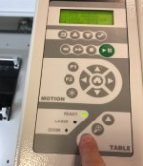
\includegraphics[height=5cm]{img/rotationseinheit/6ca5b3f580d30255d941d5c11fcb8009bef08d39.png}}
	
	-\textgreater{} \textbf{Maschine abschalten}
	
	
	-\textgreater{} Rotationsachse hinten links anlegen und den Stecker in
	die Buchse für die Rotationseinheit stecken
	
	\subsection{Nutzung}
	
	- \textgreater{} Maschine einschalten
	
	
	
	-\textgreater{} Glas einspannen
	
	{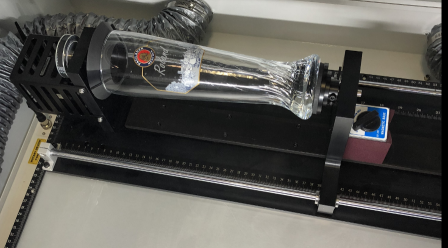
\includegraphics[height=5cm]{img/rotationseinheit/38358ef6ae653ec2e9c5f955a59b064e9fc93d55.png}}
	
	
	
	
	
	
	
	
	
	In Corel Hilfrechteck mit dem Umfang ($D \cdot \Pi$) des Glases und der Höhe
	platzieren - ist zur Orientierung.
	
	Design machen und das Ganze dann 90 Grad drehen damit die Orientierung
	des Designs mit dem Glas übereinstimmt
	
	
	
	{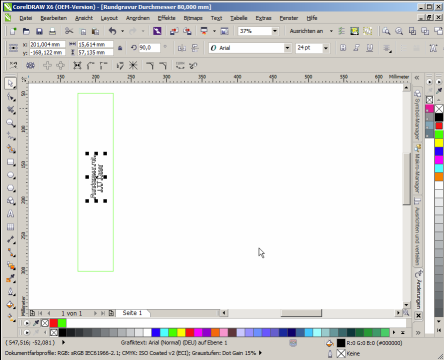
\includegraphics[height=5cm]{img/rotationseinheit/2ddfed951537c92f612bb310068bfb1863091218.png}}
	
	
	
	
	
	Position ist erst einmal unwichtig da wir mit temp Ref-Punkt arbeiten
	
	
	
	Objekt anwählen - Drucken - nur Auswahl -
	
	
	
	{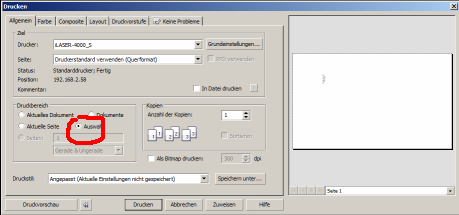
\includegraphics[height=5cm]{img/rotationseinheit/15637ec2f50b784addef4b18e06609a5e3e1a861.png}}
	
	
	
	
	
	Einstellung Laser
	
	
	
	{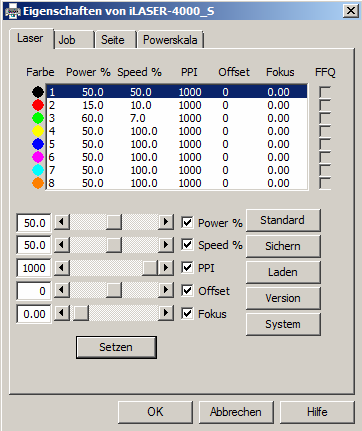
\includegraphics[height=7cm]{img/rotationseinheit/8fbb2d73cc1fb43cc120170a5d8de06295c60b70.png}}
	{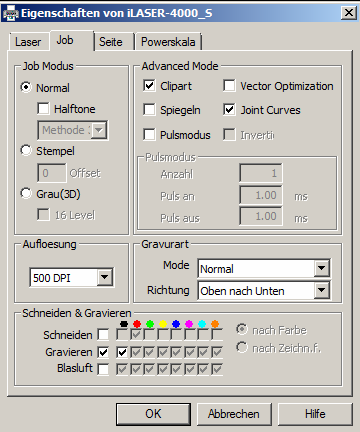
\includegraphics[height=7cm]{img/rotationseinheit/b80d0b448a255c3e0948040833bef1772f565741.png}}
	{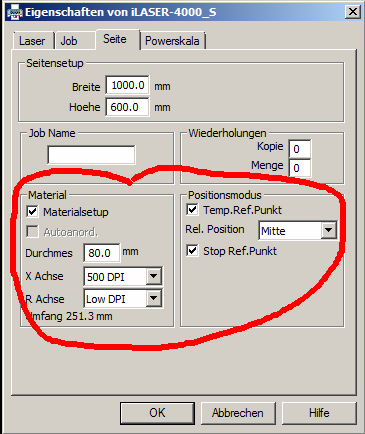
\includegraphics[height=7cm]{img/rotationseinheit/c207a27e6fec93830f6c59b31fe79151862d4ecb.png}}
	
	
	
	Durchmesser vom Glas eingeben und Optionen wie auf Abb.
	
	
	
	- \textgreater{}jetzt Drucken - damit ist die Datei im Laser und startet
	dort wo wir im Anschluss nun festlegen
	
	
	
	
	
	!!!!!!!!!!!!!!!!!! Wichtig !!!!!!!!!!!!!!!!!!!!!!
	
	
	
	-\textgreater{} vergewissern dass genügend Platz in der Höhe ist um
	Kollisionen zu vermeiden.
	
	
	
	\protect\hypertarget{Bild8}{}{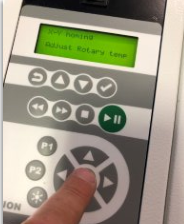
\includegraphics[height=5cm]{img/rotationseinheit/0680f038ffe19febe18861785b44851784749183.png}}
	
	
	
	-\textgreater{} Home Taset drücken
	
	-\textgreater{} Menüpunkt Adjust Rotary temp bestätigen
	
	{Laserkopf fähr nun in Zentrum Rotary Y und irgenwo in X-Achse}
	
	
	
	-\textgreater{} Mit Richtungstasten in X verfahren und Rotation
	verfahren bis di egewünschte Position zur Mittigen Ausgabe erreicht ist.
	
	{bestätigen und Menü verlassen.}
	
	
	
	- \textgreater{} Start am Laser drücken
	
	
	
	Am besten erst einen Leerlauf machen mit ausreichend DSistanz zum
	Werkstück.
	
	Erst nach korrekter Einstellung auf die Fokusdistanz gehen.
	
	
	
	Bitte Speed unter 60\% wählen, damit der Laser nicht so weit ausholt -
	es sei denn es ist ausreichend Platz da.
	
	\subsection{Ausbau}
	\textbf{Z nach ganz unten fahren}
	
	\textbf{Maschine ausschalten!}
	
	Rotationseinheit ausbauen
	
	Maschine einschalten
	
	Wabentisch einbauen, dabei auch die zwei Absaugschläuche links und rechts anschließen. Wabentisch festschrauben.
	
	\section{\nurZing Fehlerbehebung}
	In diesem Abschnitt stehen Hinweise zu häufigen Fehlern speziell für den Epilog Zing. Siehe auch \cref{sec:fehler-allgemein} für allgemeine Hinweise.
	
	\subsection{Windows-Druckertreiber}	
	\subsubsection{Probleme mit 1000dpi}
	Verwendet man die Einstellung 1000dpi können Fehler auftreten. Meist hängt der Druckjob ewig fest oder die Data-Leuchte geht nicht mehr aus. Dieses Problem lässt sich nur durch Neustarten aller Geräte lösen. Also zuerst die VM neustarten, dann den Lasercutter. Der Druckjob muss erneut geschickt werden. Jetzt sollten entweder 500dpi genutzt werden oder VisiCut.
	
	\subsubsection{Data leuchtet ständig, Job hält an}
	Data soll vor dem Starten eines Jobs ausgegangen sein! Ansonsten hält der Job manchmal irgendwann in der Mitte an.
	
	Das bedeutet, dass Windows sich verschluckt hat und den Rest des Jobs nicht senden will. Stop drücken, eine Epilog-Gedenkminute lang warten und beten, dass Data spontan ausgeht. Ansonsten auf die harte Tour: Stop, Reset, ggf. den Nullpunkt markieren damit man ihn wiederfindet. Laser ausschalten, Druckauftrag abbrechen (in der Windows-VM über das Druckersymbol in der Taskleiste), Windows-VM über Startmenü neustarten, Laser wieder anschalten.
	
	\subsection{Mechanik}
	Bitte führe Wartungen an der Mechanik nur dann durch, wenn du weißt, was du tust!
	
	\subsubsection{Gravur zittrig}
	\begin{wrapfigure}{r}{2cm}
		\vspace{-50pt} %WORKAROUND: Nicht so viel leerer weißer Platz
		\includegraphics[width=2cm]{./img/fehler-umlenkspiegel.png}
		\vspace{-20pt} %WORKAROUND: Nicht so viel leerer weißer Platz
	\end{wrapfigure}
	Wenn es so aussieht wie auf dem Bild: Umlenkspiegel und Linse festschrauben.
	
	\subsubsection{Fokusprobleme}
	Ein falscher Fokus äußert sich dadurch, dass das Schneiden schlecht und die Gravur nur schwach und verrauscht funktioniert. Prüfe zuerst mit dem Fokuspendel, ob der Fokus richtig eingestellt ist.
	
	Wenn es trotzdem nicht funktioniert, kann es sein dass die Länge des Fokuspendels nicht mehr stimmt. Dies kann mit einem Test überprüft werden:
	
	Zum Testen wird VisiCut gestartet und ein spezielles LaserScript geladen: Datei \pfeil Beispiele \pfeil vordefiniert \pfeil LaserScript \pfeil Focustest und auf \enquote{Papier 80g, alles cut} gestellt.
	Als nächste muss ein A3 Blatt Papier im Querformat (oder 2x A4 nebeneinander) eingelegt und auf die Materialoberseite fokussiert werden.
	
	Das Script testet auf dem Papier verschiedene Fokusabstände und wenn der Fokus so wie eingestellt stimmt, sollte der dünnste, präziseste Schnitt bei Höhe 0 vorliegen.
	
	
	\subsubsection{Material wird in einer Ecke nicht durchtrennt}
	Es kann vorkommen, dass Material in einer der Ecken nicht richtig durchtrennt wird trotz richtig eingestelltem Fokus. Dies liegt meistens daran, dass der Tisch schief steht.
	
	Zur Behebung wird der Tisch ausgebaut. (Dazu den Arm bei ausgeschaltenem X/Y aus dem Weg schieben.) Meist liegt etwas in einer der beiden Vertiefungen der unteren Lineale. Diese gegebenenfalls reinigen. Zum Abschluss den Tisch wieder gerade einsetzen, sicher stellen, dass er in den Vertiefungen sitzt und mit sanftem Druck bis zum Boden drücken.
	
	\subsubsection{Wagen macht schabende Geräusche}
	Der blaue Wagen läuft auf drei Rollen im schwarzen Arm. Falls der Wagen nicht korrekt eingesetzt ist, lässt er sich nur schwergängig unter schabenden Geräuschen bewegen. Um dies zu beheben drückt man die Klammer, die das Rad auf der dem Benutzer abgewandten Seite hält zusammen. Jetzt lässt sich der Wagen bewegen. Eigentlich müsste er die richtige Position \enquote{von selbst} finden. Eventuell ist auch der Metallträger, der am Riemen befestigt ist im Arm verklemmt. Um dies zu beseitigen, löst man die zwei Schrauben auf dem Wagen, die den Träger fest halten und montiert die Anlage neu.
	
	\subsection{Laserröhre}
	\subsubsection{unterbrochene Schnittkanten}
	Wenn der Laser zu heiß wird, scheint er einfach den Strahl für einen kurzen Moment abzuschalten. Dies zeigt sich dann in einer mehrfach unterbrochenen Schnittlinie. Die einzelnen \enquote{Wiedereinstiche} liegen dabei direkt nebeneinander. Eine Lösung scheint zu sein, sicherzustellen, dass der Laser auf der linken Seite kühle Luft ansaugt und dort kein Dreck ist.
	\subsubsection{Leistungseinbrüche}
	Wenn der Laser für ein vernünftiges Ergebnis deutlich höhere Leistungseinstellungen als gewöhnlich benötigt, ist das ein Hinweis auf eine verschmutzte Linse. Nach Abschalten des roten Lasers, kann man den Verschmutzungsgrad der Linse mit einem Spiegel überprüfen. Die Reinigungsprozedur ist in \ref{linsenreinigung} auf Seite \pageref{linsenreinigung} beschrieben. Bei schlechten Lichtverhältnissen kann es auch sein, dass eine Verschmutzung erst nach Ausbau der Linse erkennbar ist.
	\subsubsection{Müdigkeit}
	Wenn der Laser mehrere Tage nicht genutzt wird, ist er in der ersten halben Stunde etwas müde -- wahrscheinlich ist die Ionisierung der Laserröhre dann noch nicht so gut. Die Röhre hat dann manchmal Probleme zu zünden, sodass manche Stellen nicht oder nur teilweise gelasert werden. Nach etwas Benutzung verschwindet das Problem von selber.
	
	
	\newpage
	\ccLicense{lasercutter-einweisung}{Einweisung Lasercutter}
	
\end{document}
